\chapter{Годограф Найквиста}

В соответствии с вариантом задания, придумаем три объекта пятого порядка 1 полюс передаточных функций которых 
вещественный, а остальные 4 комплексно-сопряженные.

\section{Объект 1}
Первая передаточная функция должна иметь 4 неустойчивых полюса у разомкнутой системы и 4 неустойчивых полюса у замкнутой.

Если общий вид передаточной функции разомкнутой системы имеет вид:
\[
W(s) = \frac{R(s)}{Q(s)}
\]

То передаточная функция замкнутой системы имеет вид:
\[
W_\text{з}(s) = \frac{W(s)}{1 + W(s)} = \frac{R(s)}{Q(s) + R(s)}
\]

Обозначим \(Q(s) + R(s)\) как \(D(s)\), тогда передаточная функция замкнутой системы примет вид:
\[
W(s) = \frac{R(s)}{D(s)}
\]

Теперь мы можем составить выражения для \(Q(s)\) и \(D(s)\) исходя из условий задачи,
а затем выразить R(s) и передаточную функцию разомкнутой системы:
\[
Q(s) = (s+1)(s-1-i)(s-1+i)(s-2-i)(s-2+i)
\]
\[
D(s) = (s+2)(s-1-2i)(s-1+2i)(s-2-2i)(s-2+2i)
\]
\[
R(s) = D(s) - Q(s) = s^4 + 9s^2 - 24s +70
\]
\[
W(s) = \frac{s^4 + 9s^2 - 24s +70}{(s+1)(s-1-i)(s-1+i)(s-2-i)(s-2+i)}
\]

Теперь построим карту полюсов и нулей передаточной функции разомкнутой и замкнутой системы:
\begin{figure}[H]
    \centering
    \begin{minipage}{0.45\textwidth}
        \centering
        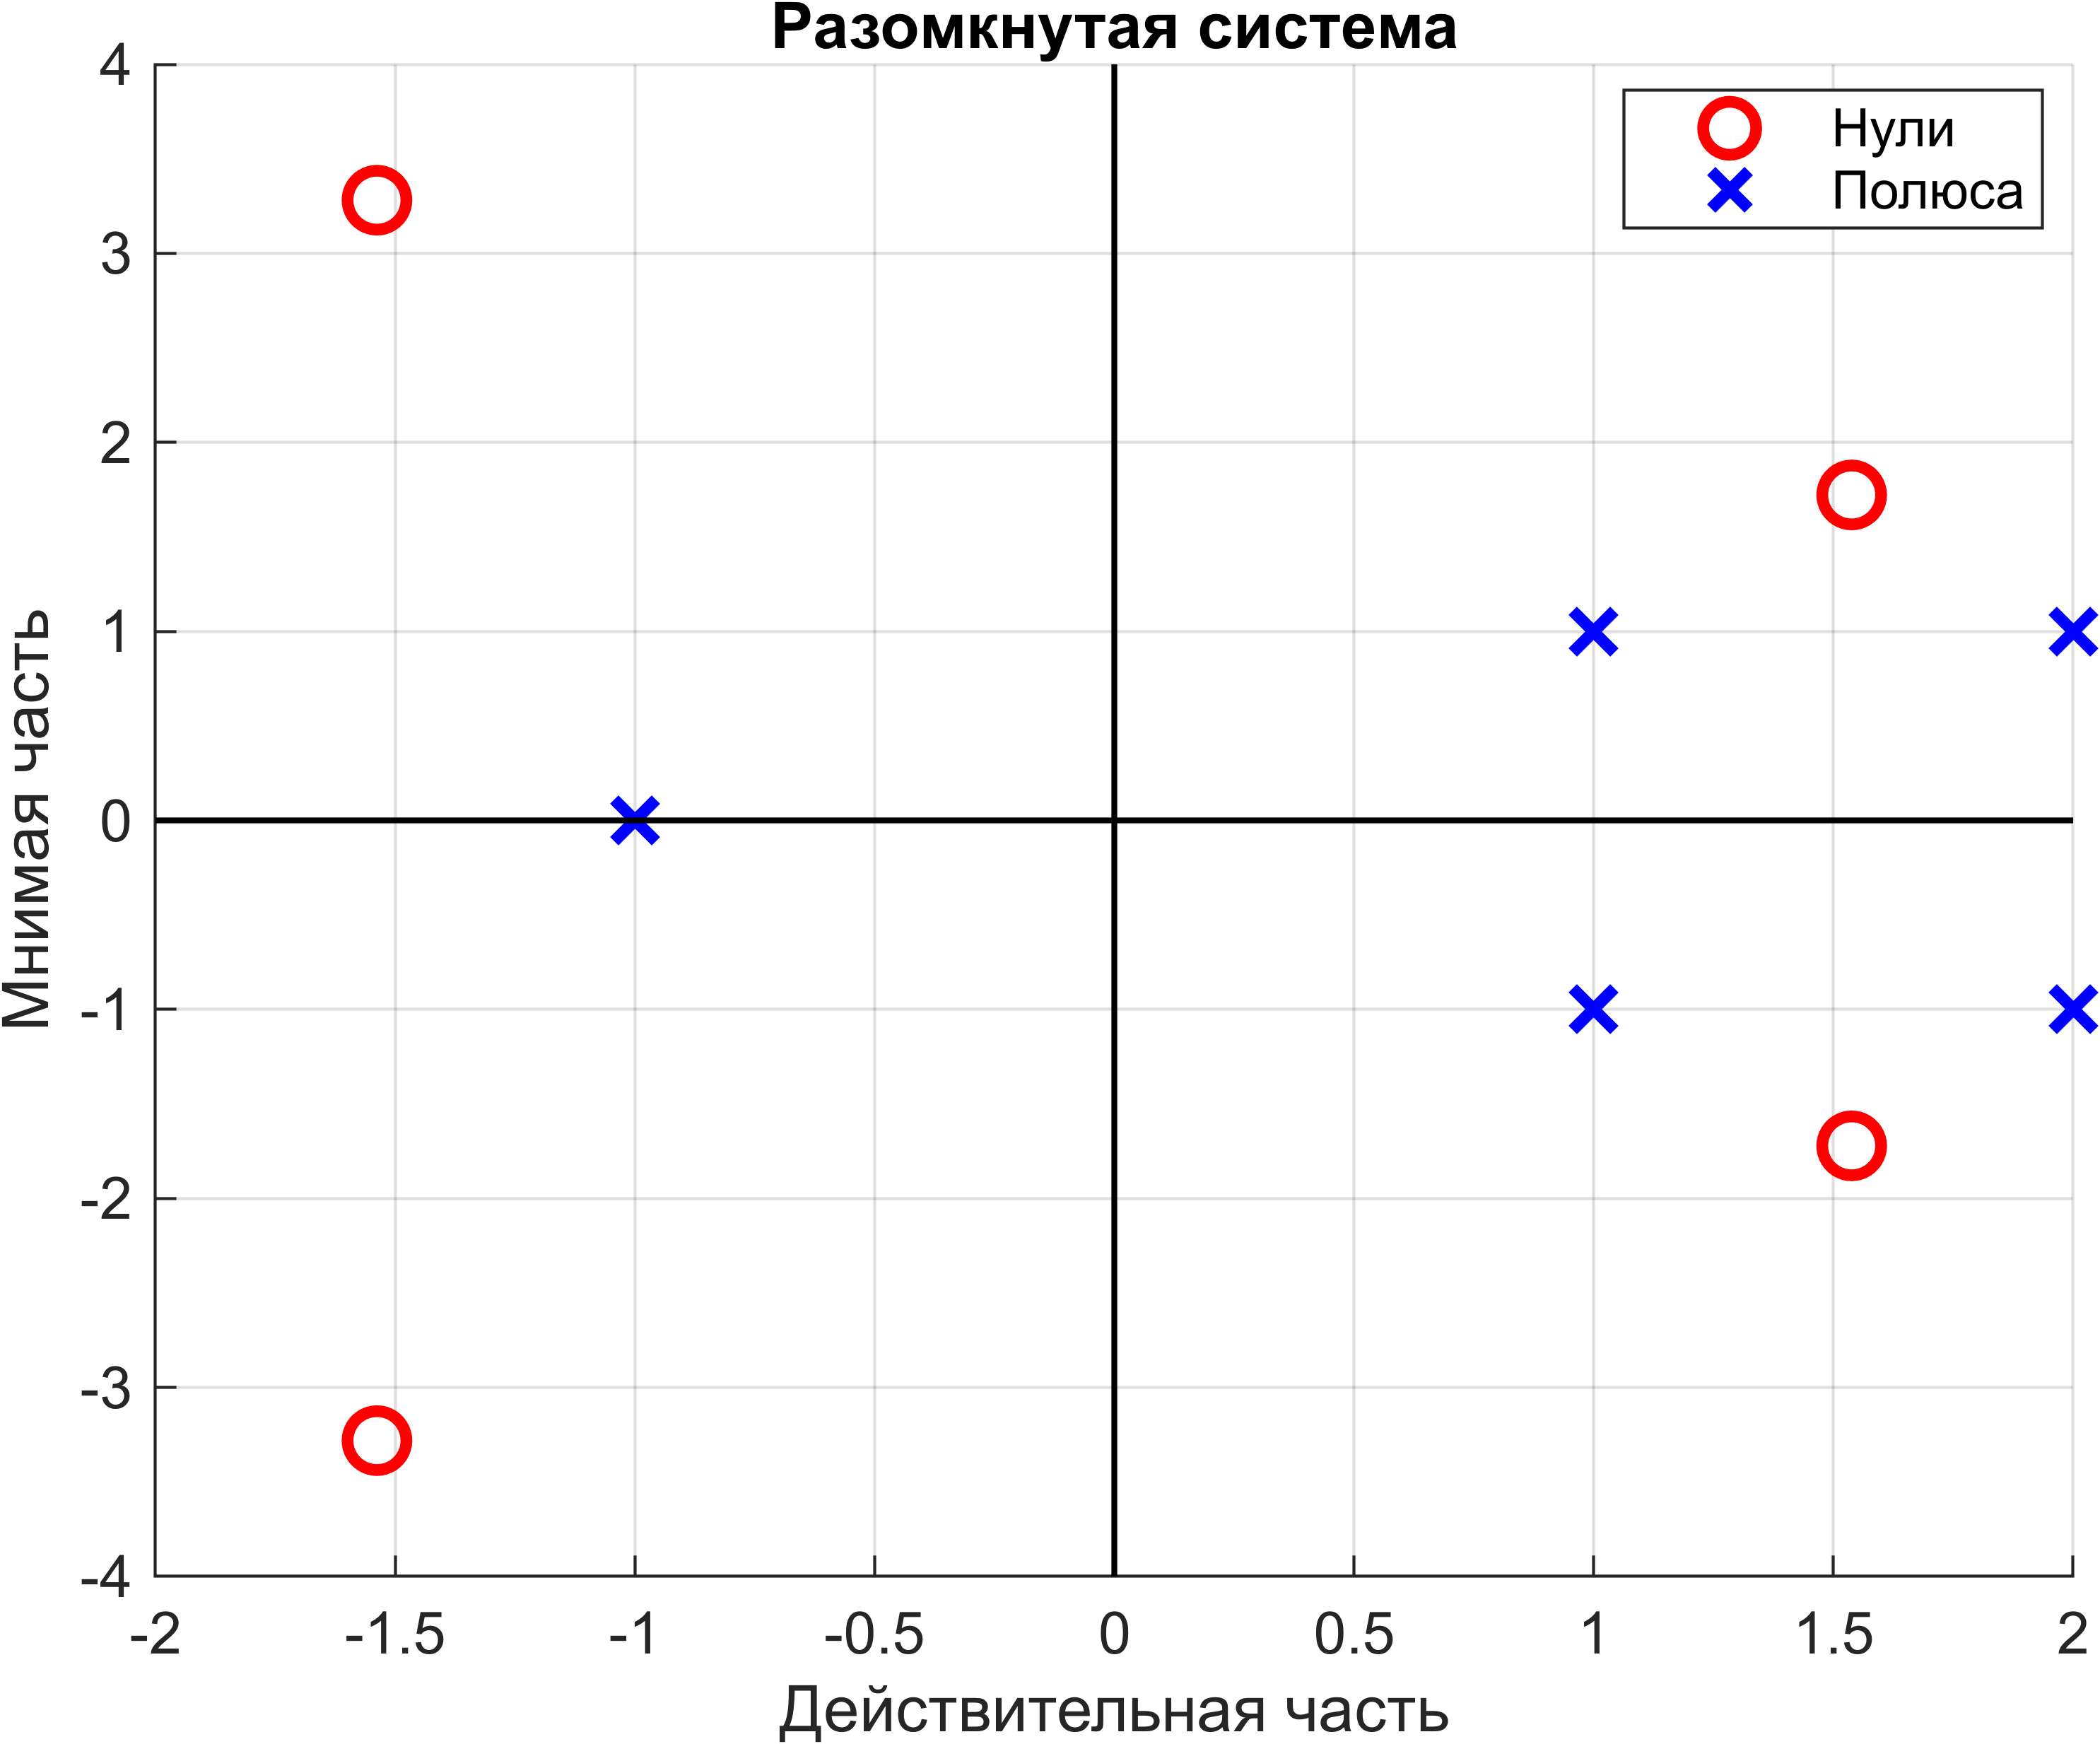
\includegraphics[width=1\textwidth, trim={0cm 0cm 0cm 0cm}]{../images/1_1_map_ol.png}
    \end{minipage}
    \hfill
    \begin{minipage}{0.45\textwidth}
        \centering
        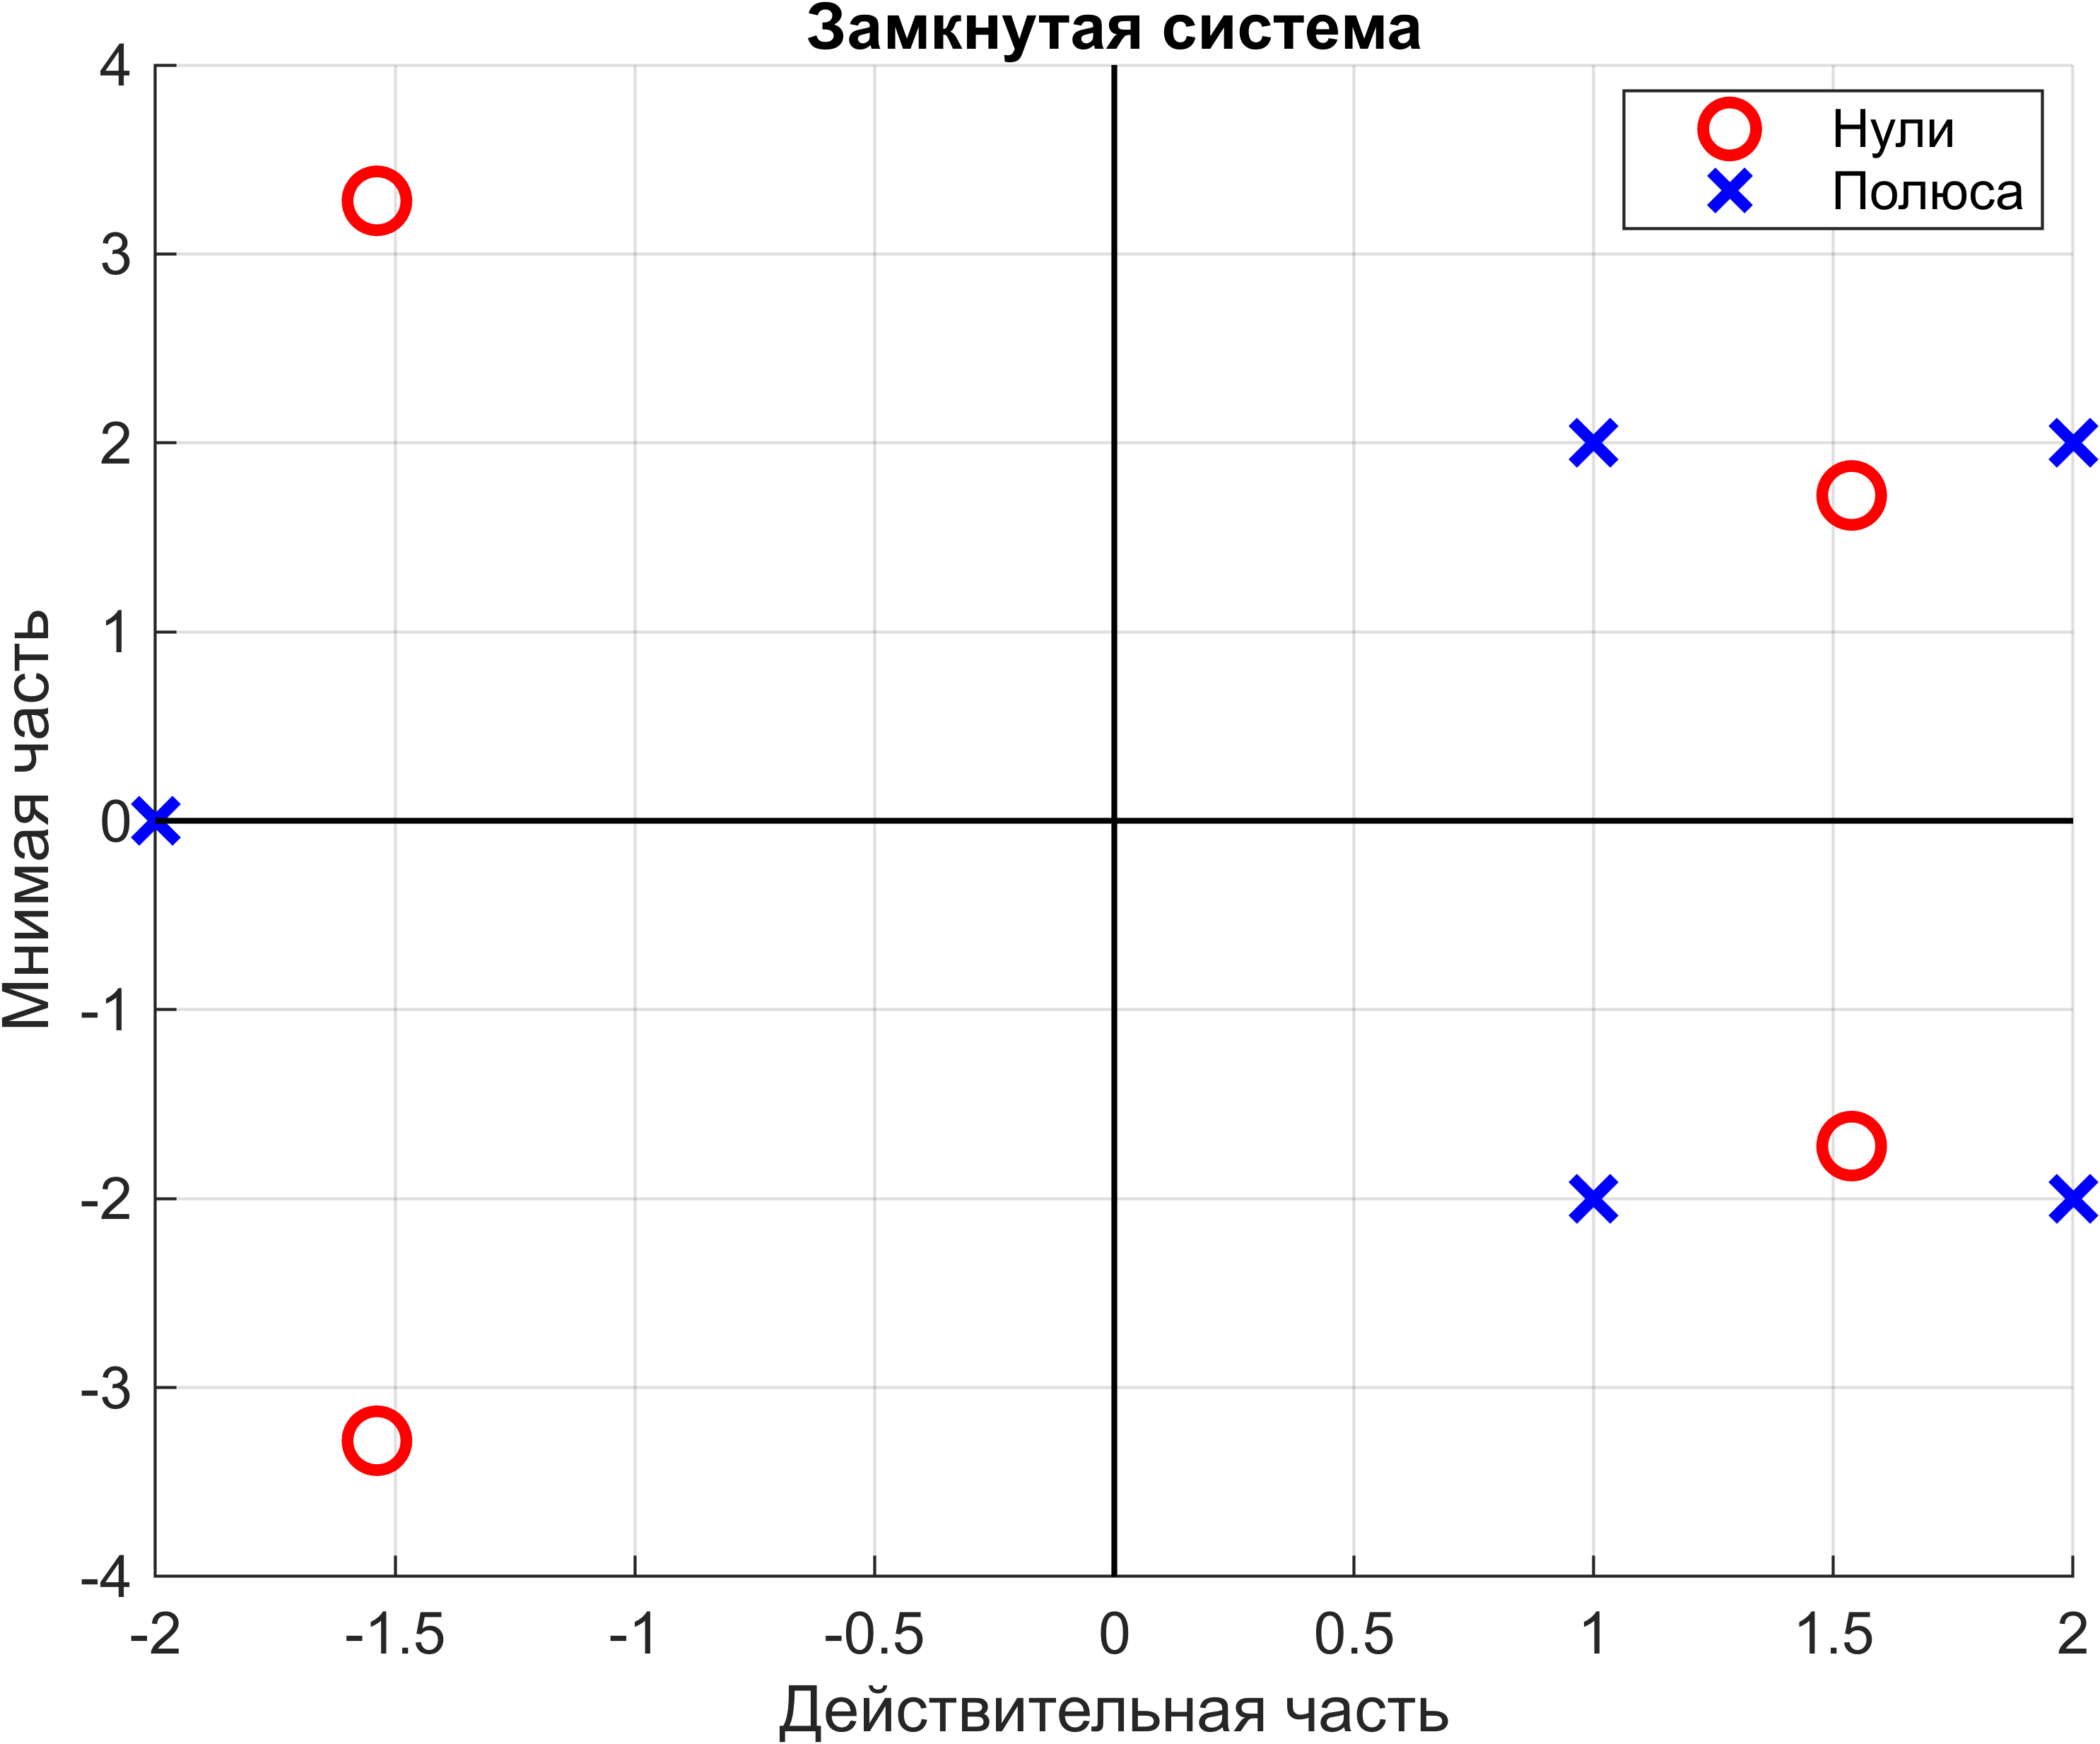
\includegraphics[width=1\textwidth, trim={0cm 0cm 0cm 0cm}]{../images/1_1_map_cl.png}
    \end{minipage}
    \caption{Карта полюсов и нулей разомкнутой и замкнутой системы}
\end{figure}

Теперь построим переходные характеристики разомкнутой и замкнутой системы:
\begin{figure}[H]
    \centering
    \begin{minipage}{0.45\textwidth}
        \centering
        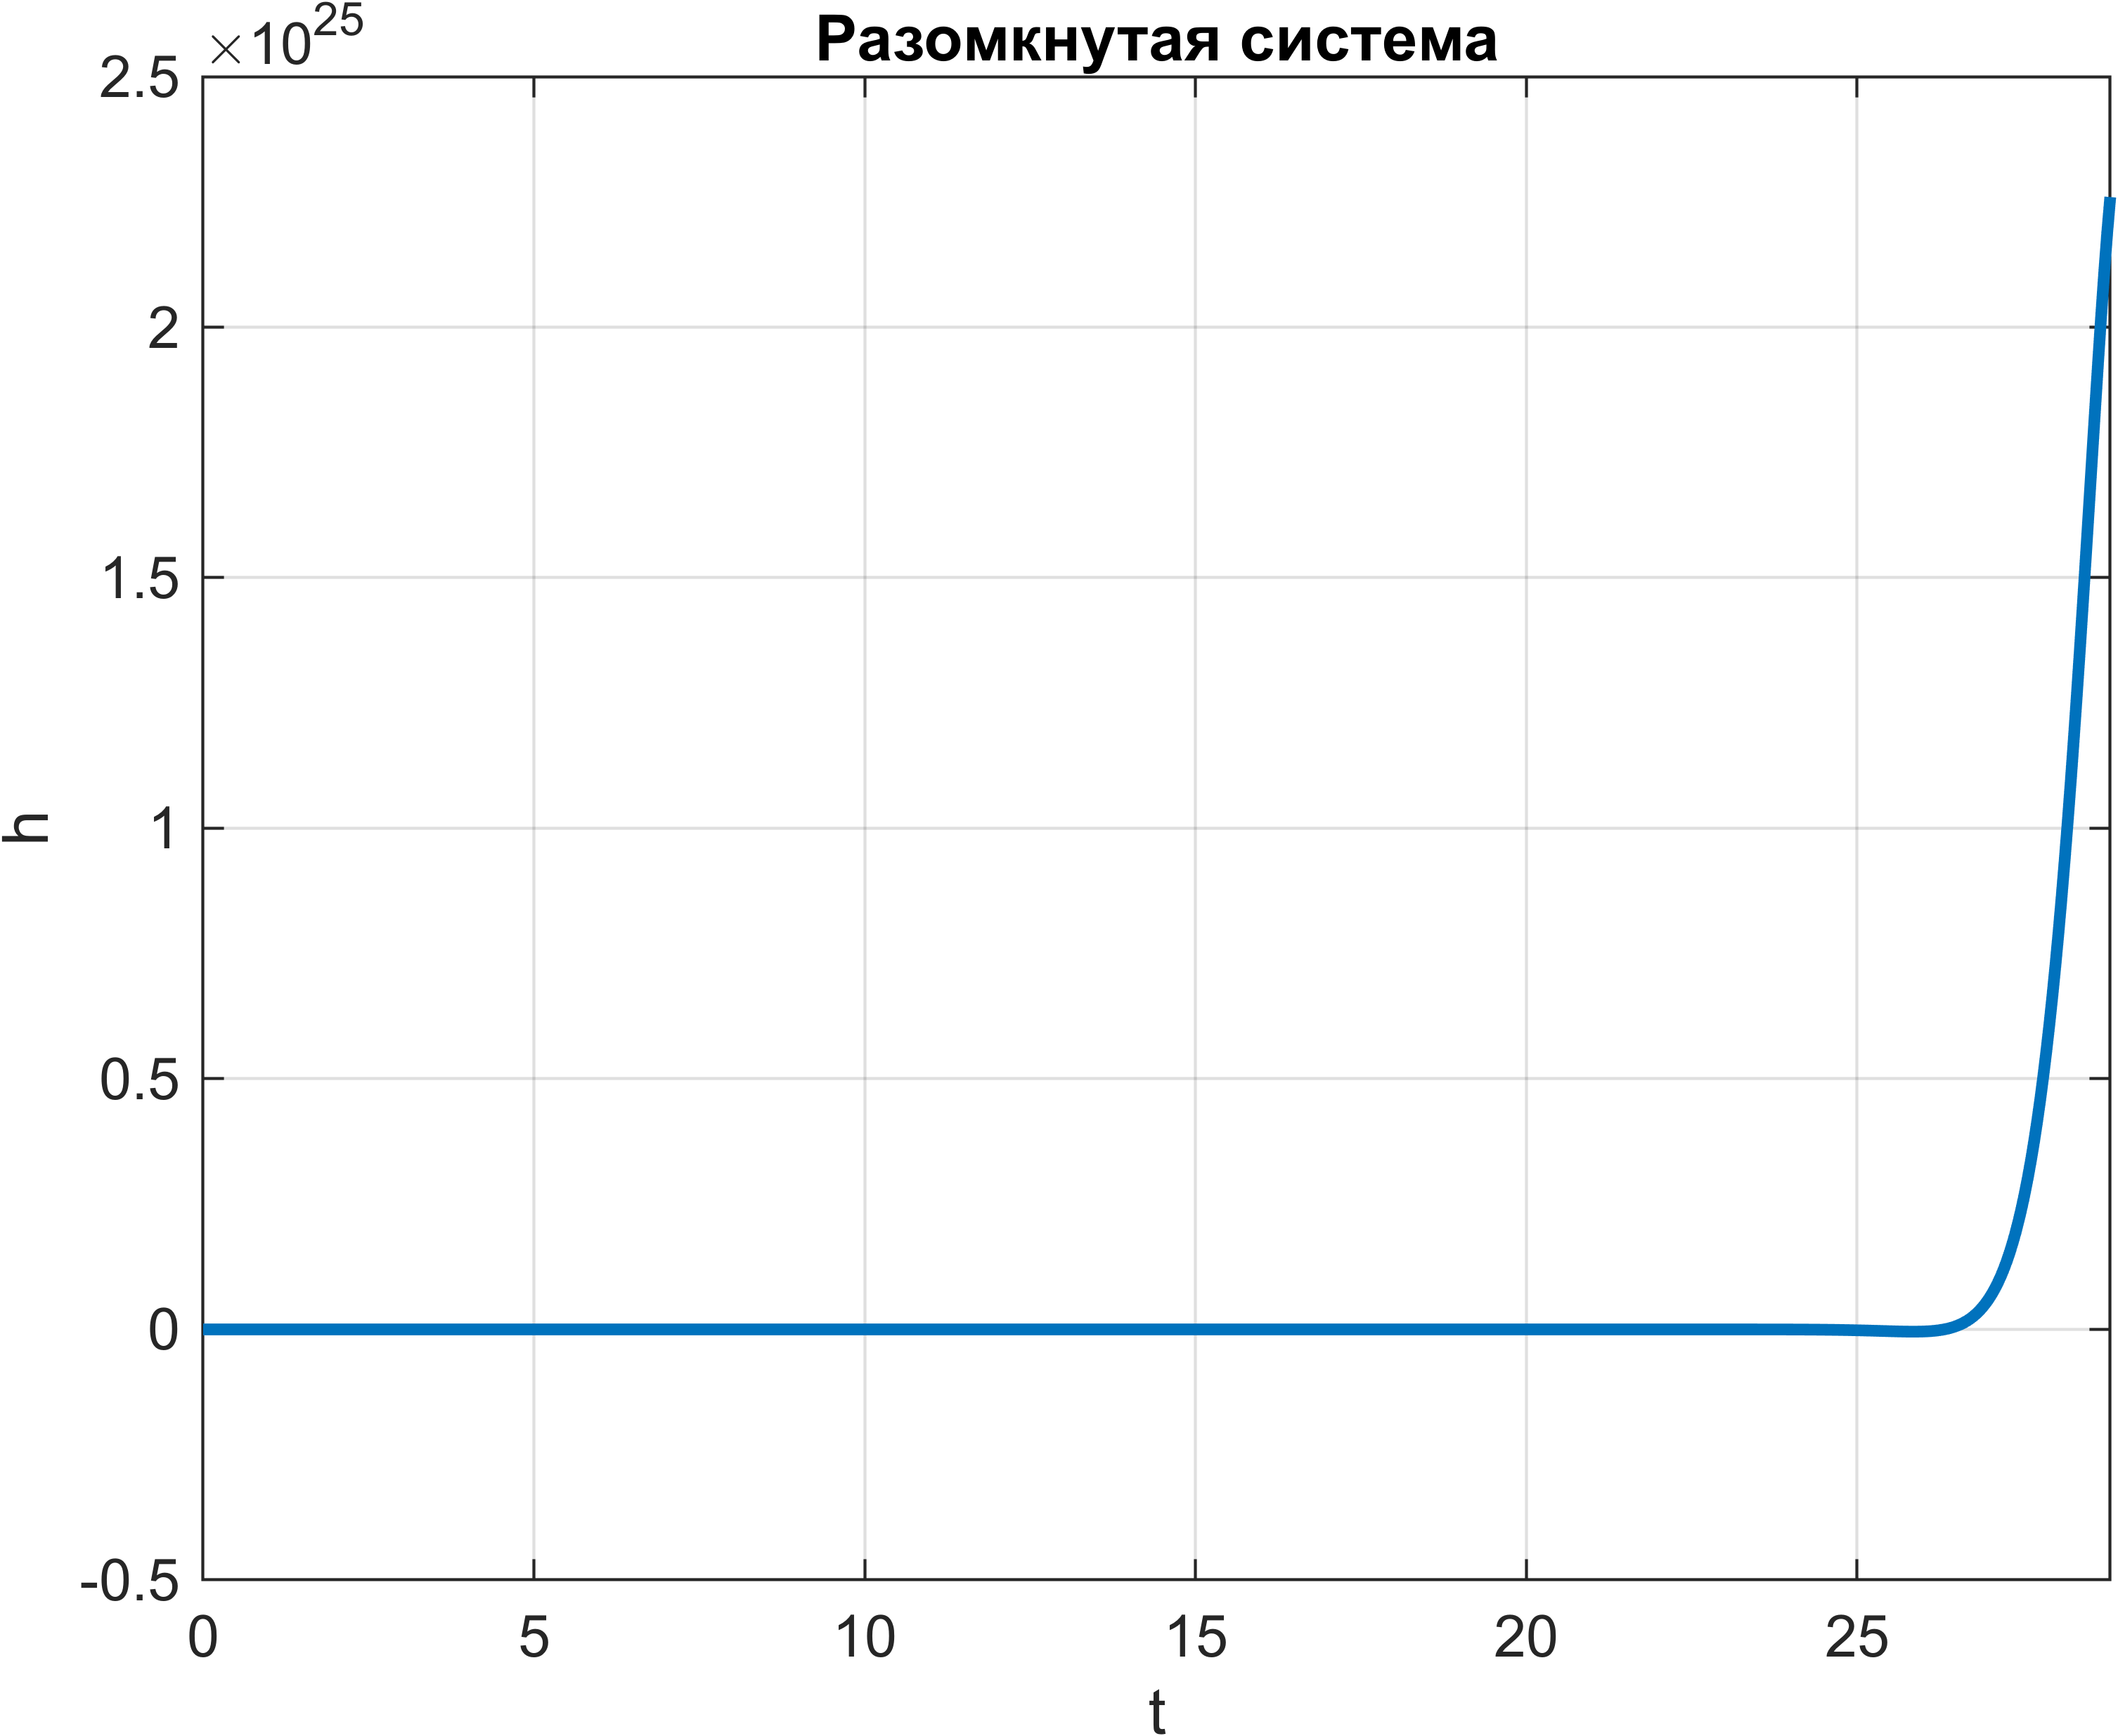
\includegraphics[width=1\textwidth, trim={0cm 0cm 0cm 0cm}]{../images/1_1_h_ol.png}
    \end{minipage}
    \hfill
    \begin{minipage}{0.45\textwidth}
        \centering
        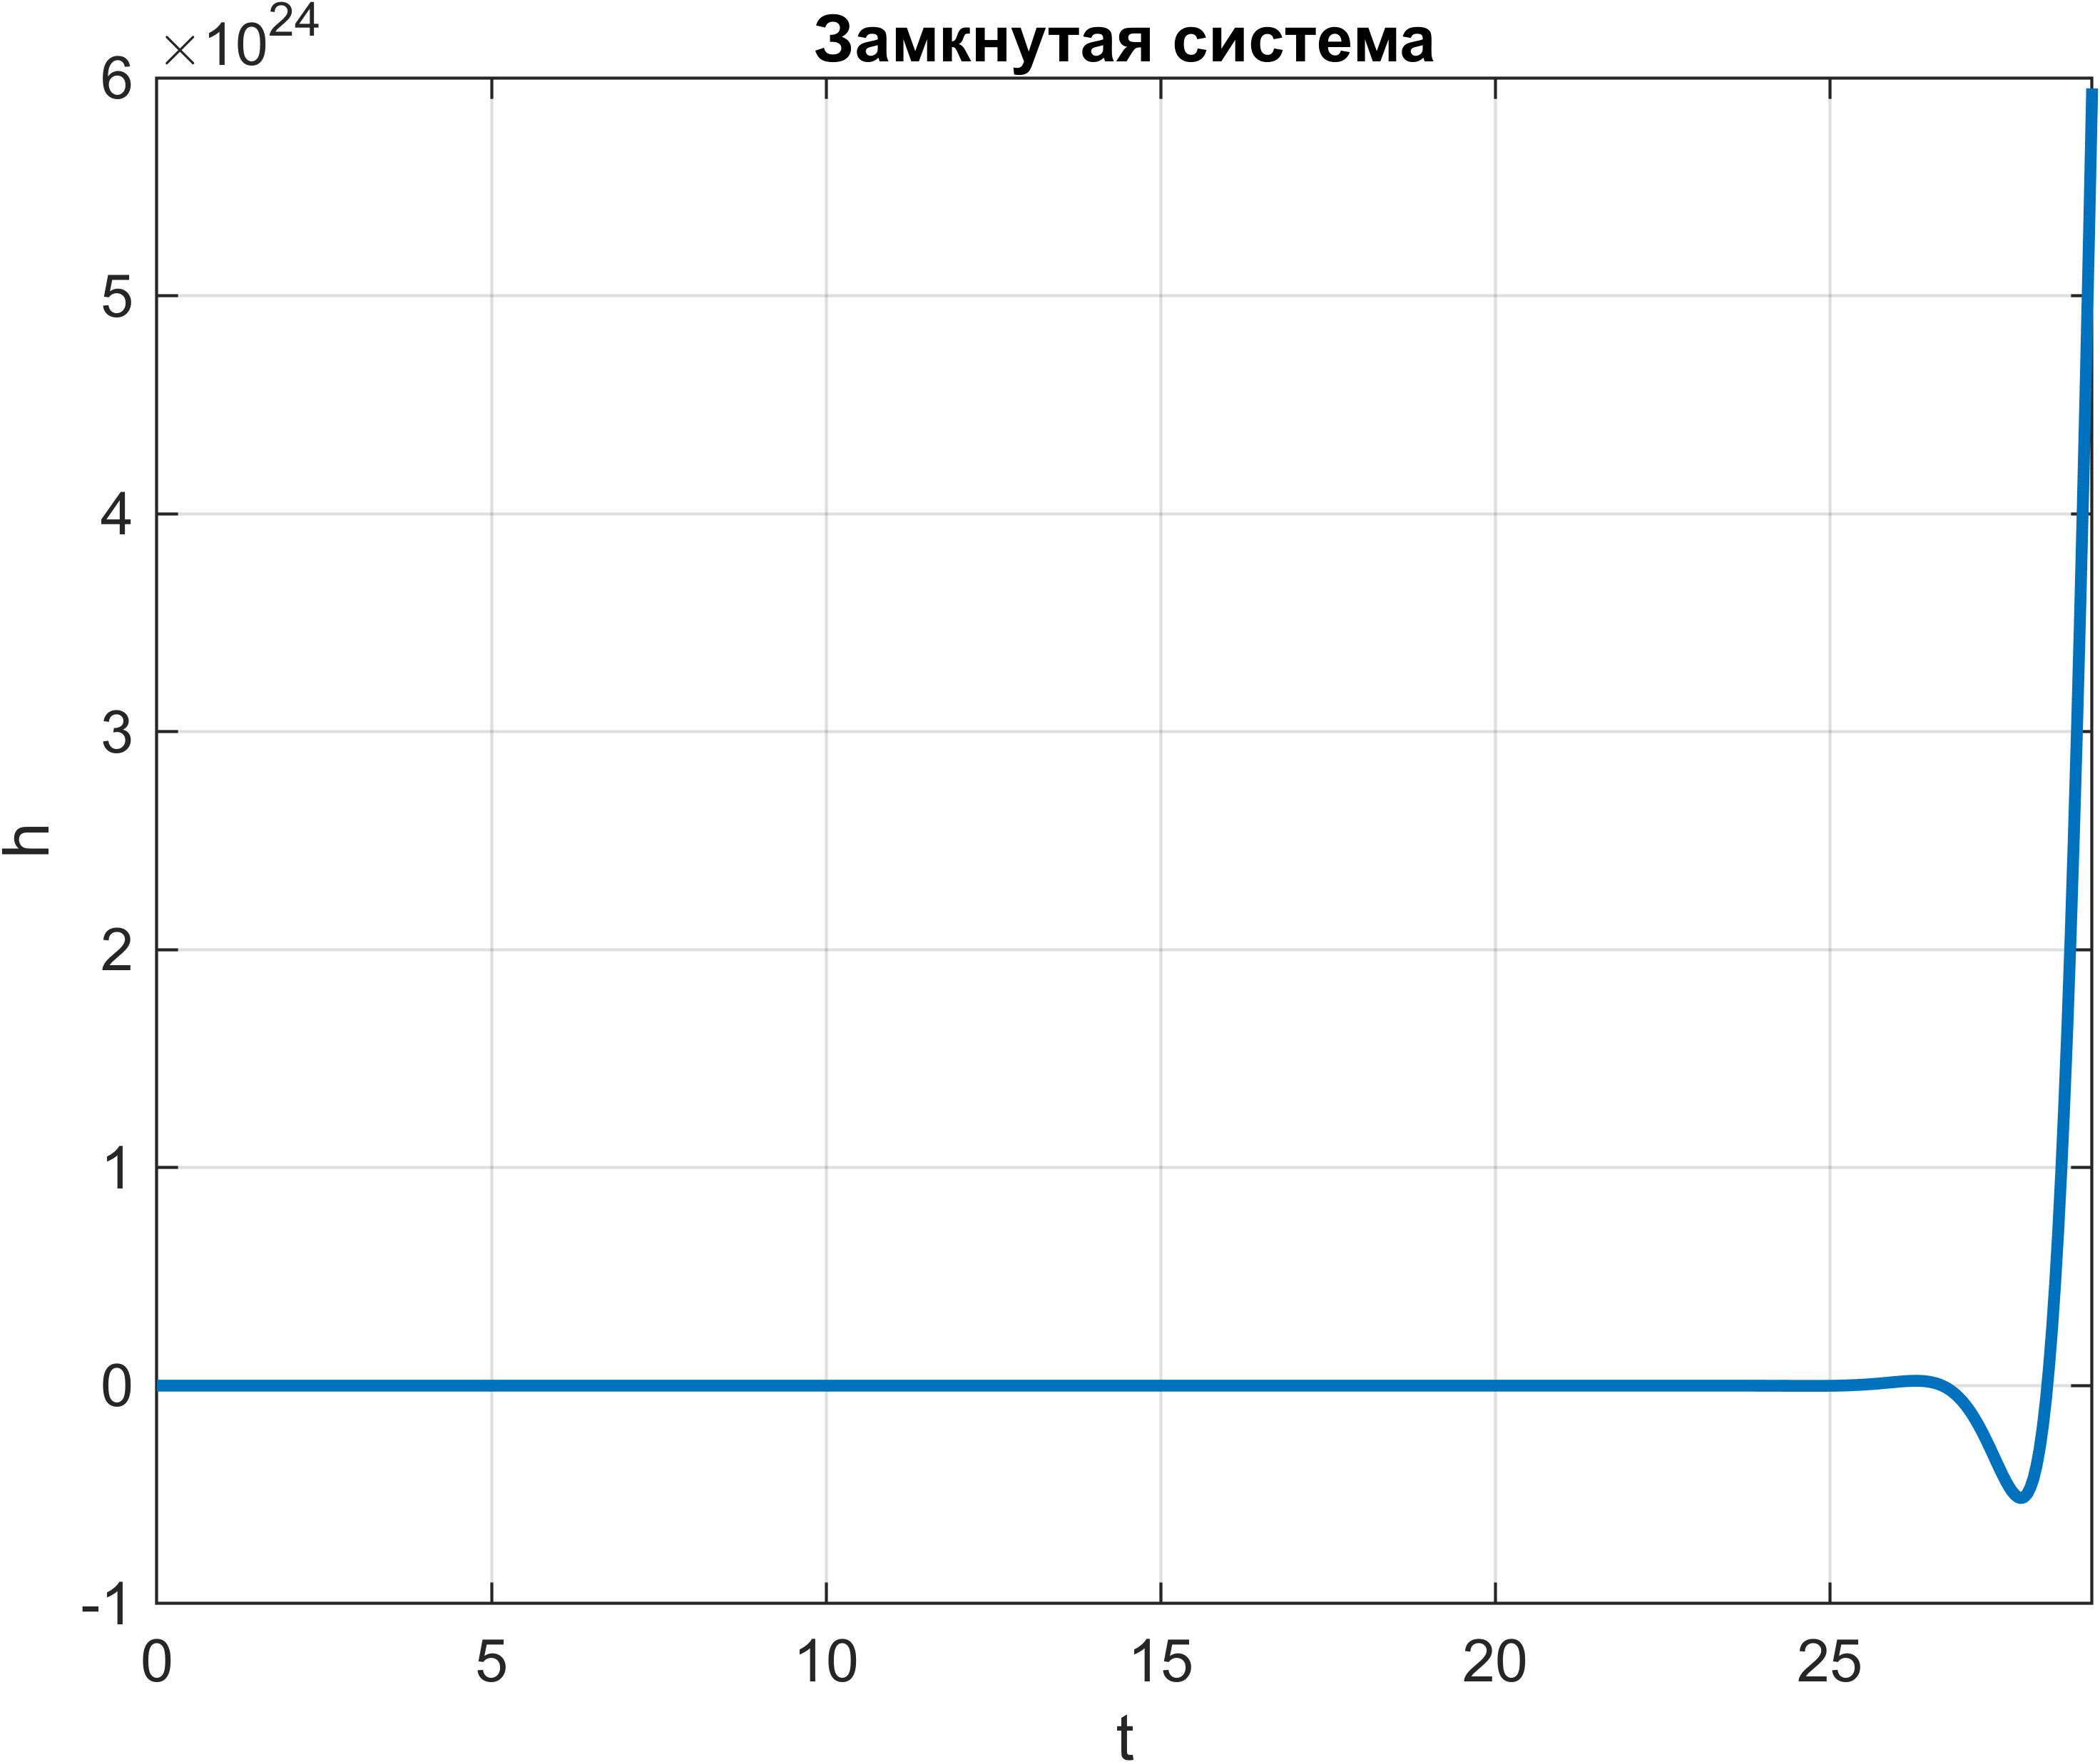
\includegraphics[width=1\textwidth, trim={0cm 0cm 0cm 0cm}]{../images/1_1_h_cl.png}
    \end{minipage}
    \caption{Переходные характеристики разомкнутой и замкнутой системы}
\end{figure}

Годограф Найквиста для данной передаточной функции:
\begin{figure}[H]
    \centering
    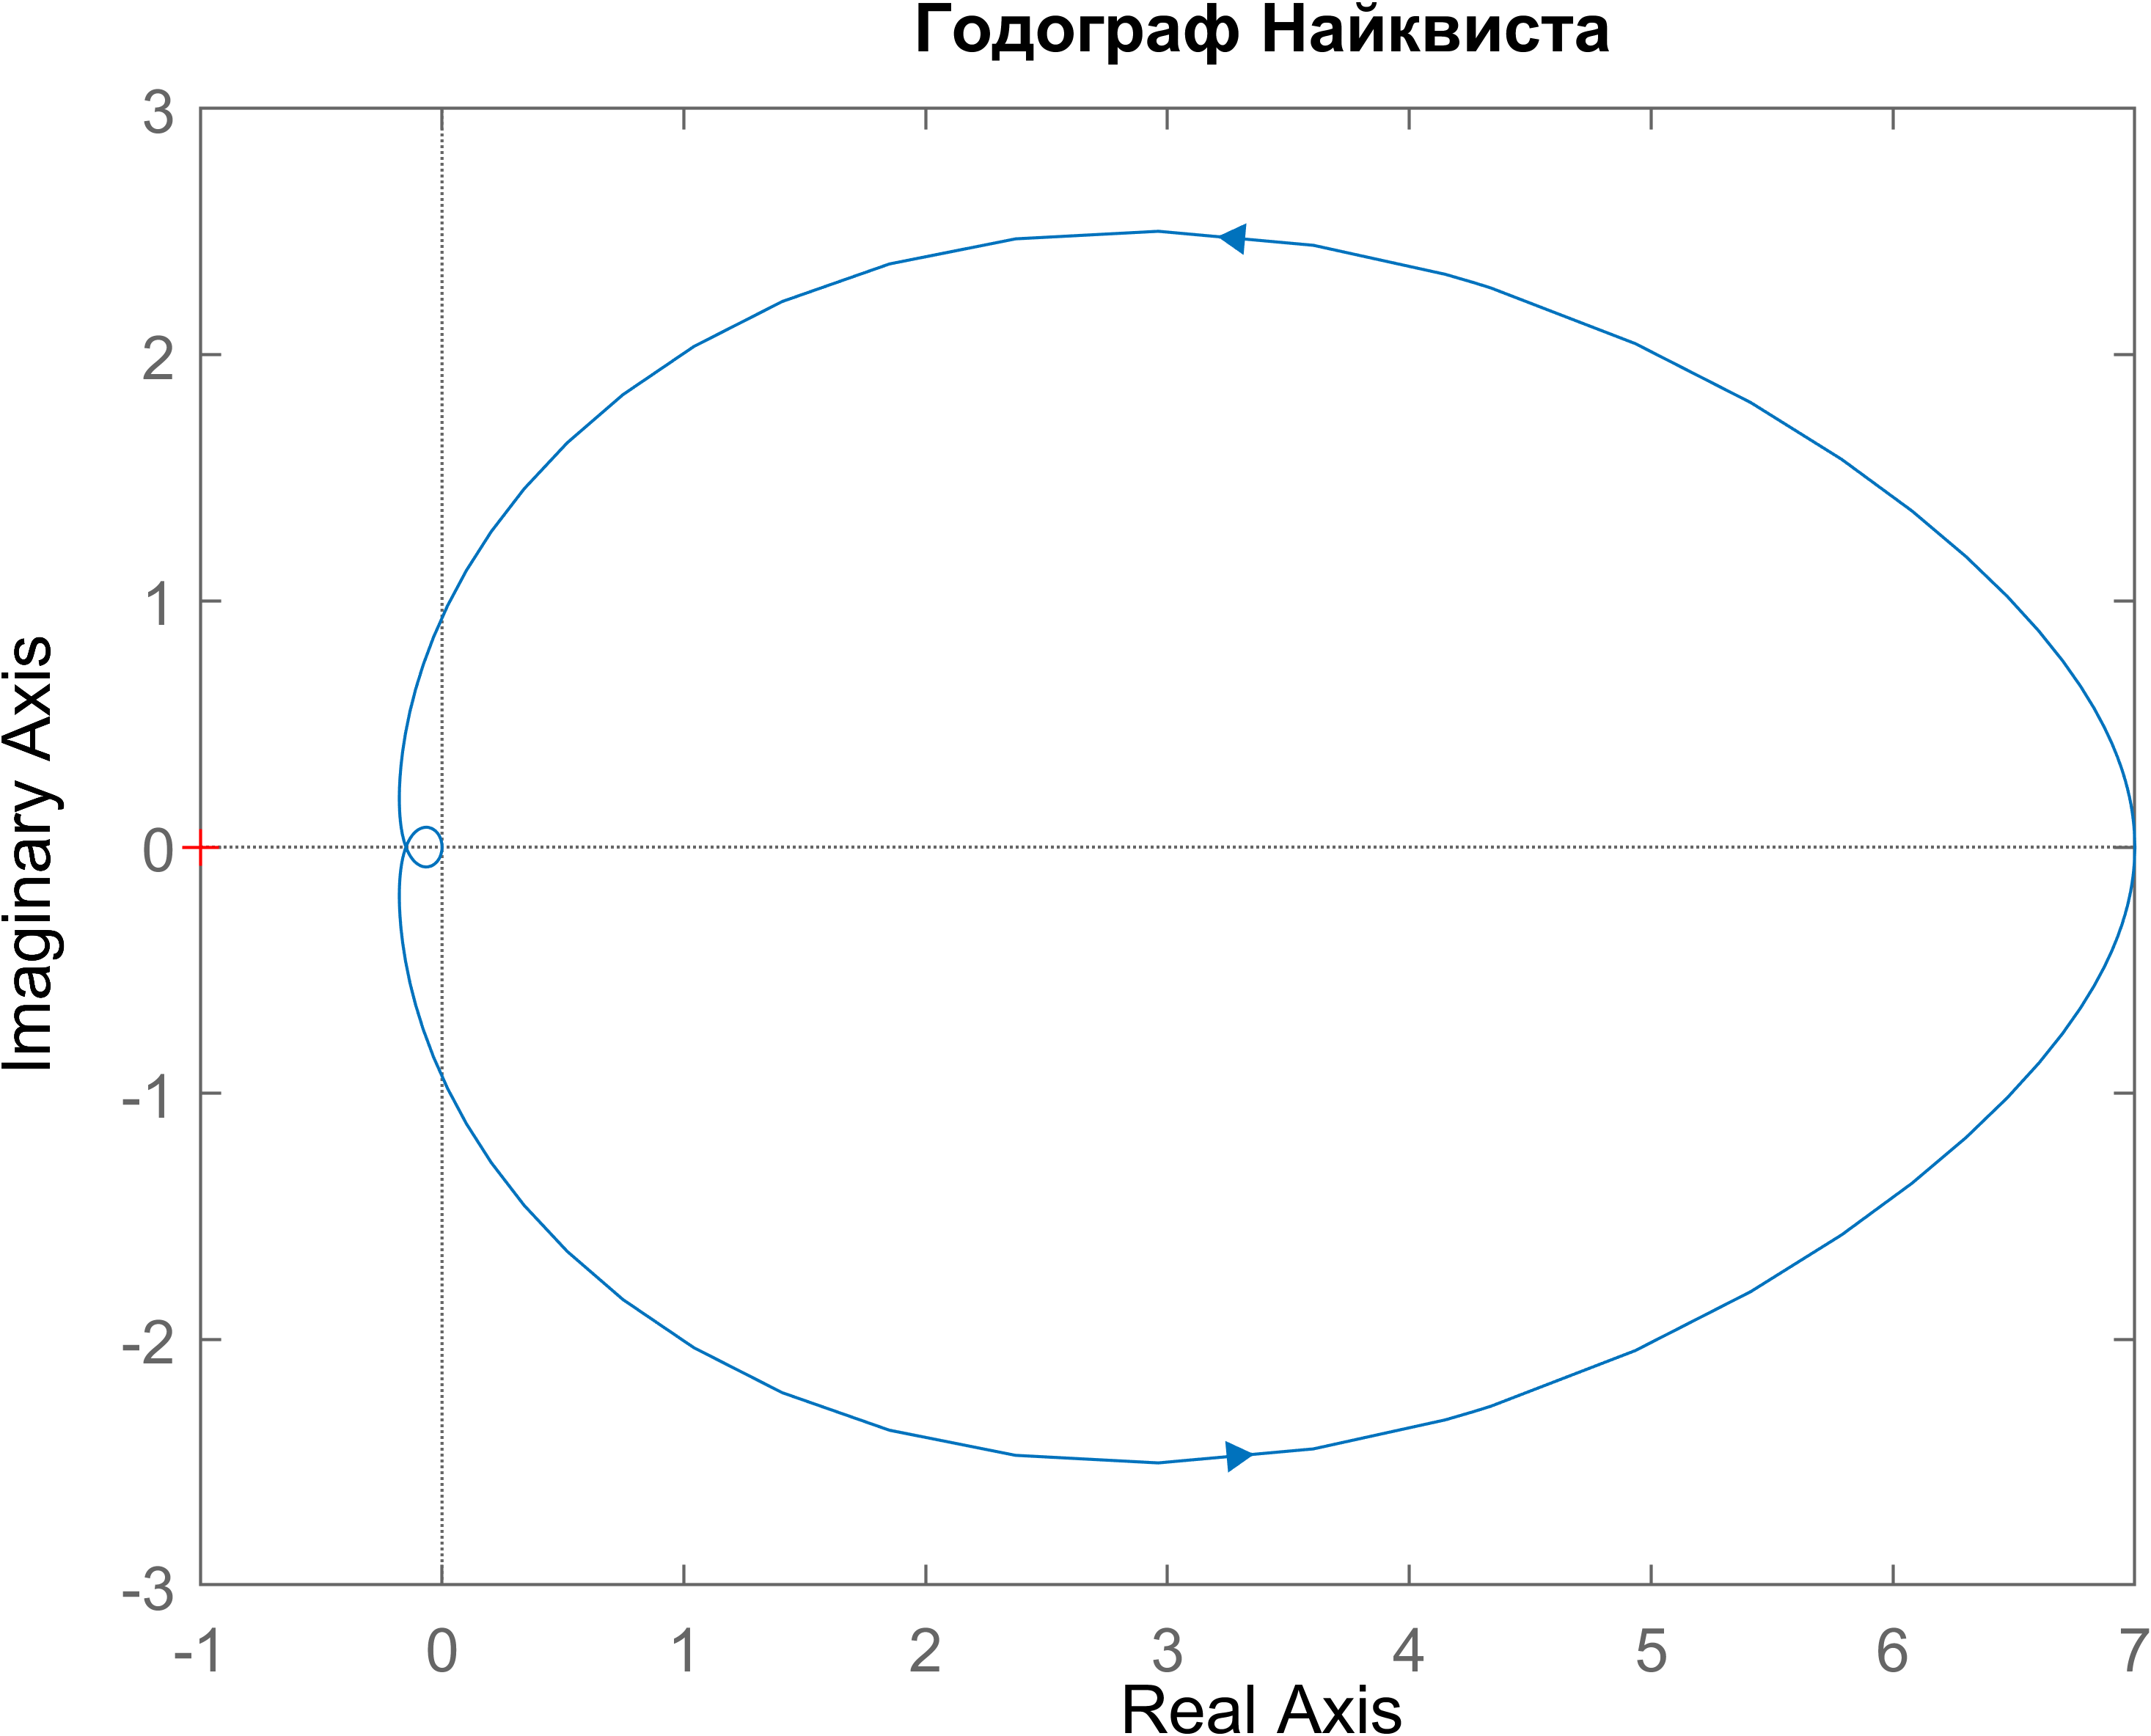
\includegraphics[width=0.7\textwidth, trim={0cm 0cm 0cm 0cm}]{../images/1_1_hod.png}
    \caption{Годограф Найквиста}
\end{figure}

Как видим, годограф не совершает оборотов вокруг точки (-1, 0). Это соотносится с критерием Найквиста, так как
количество неустойчивых полюсов не изменилось при замыкании системы.

Рассмотрим ЛАФЧХ для данной передаточной функции:
\begin{figure}[H]
    \centering
    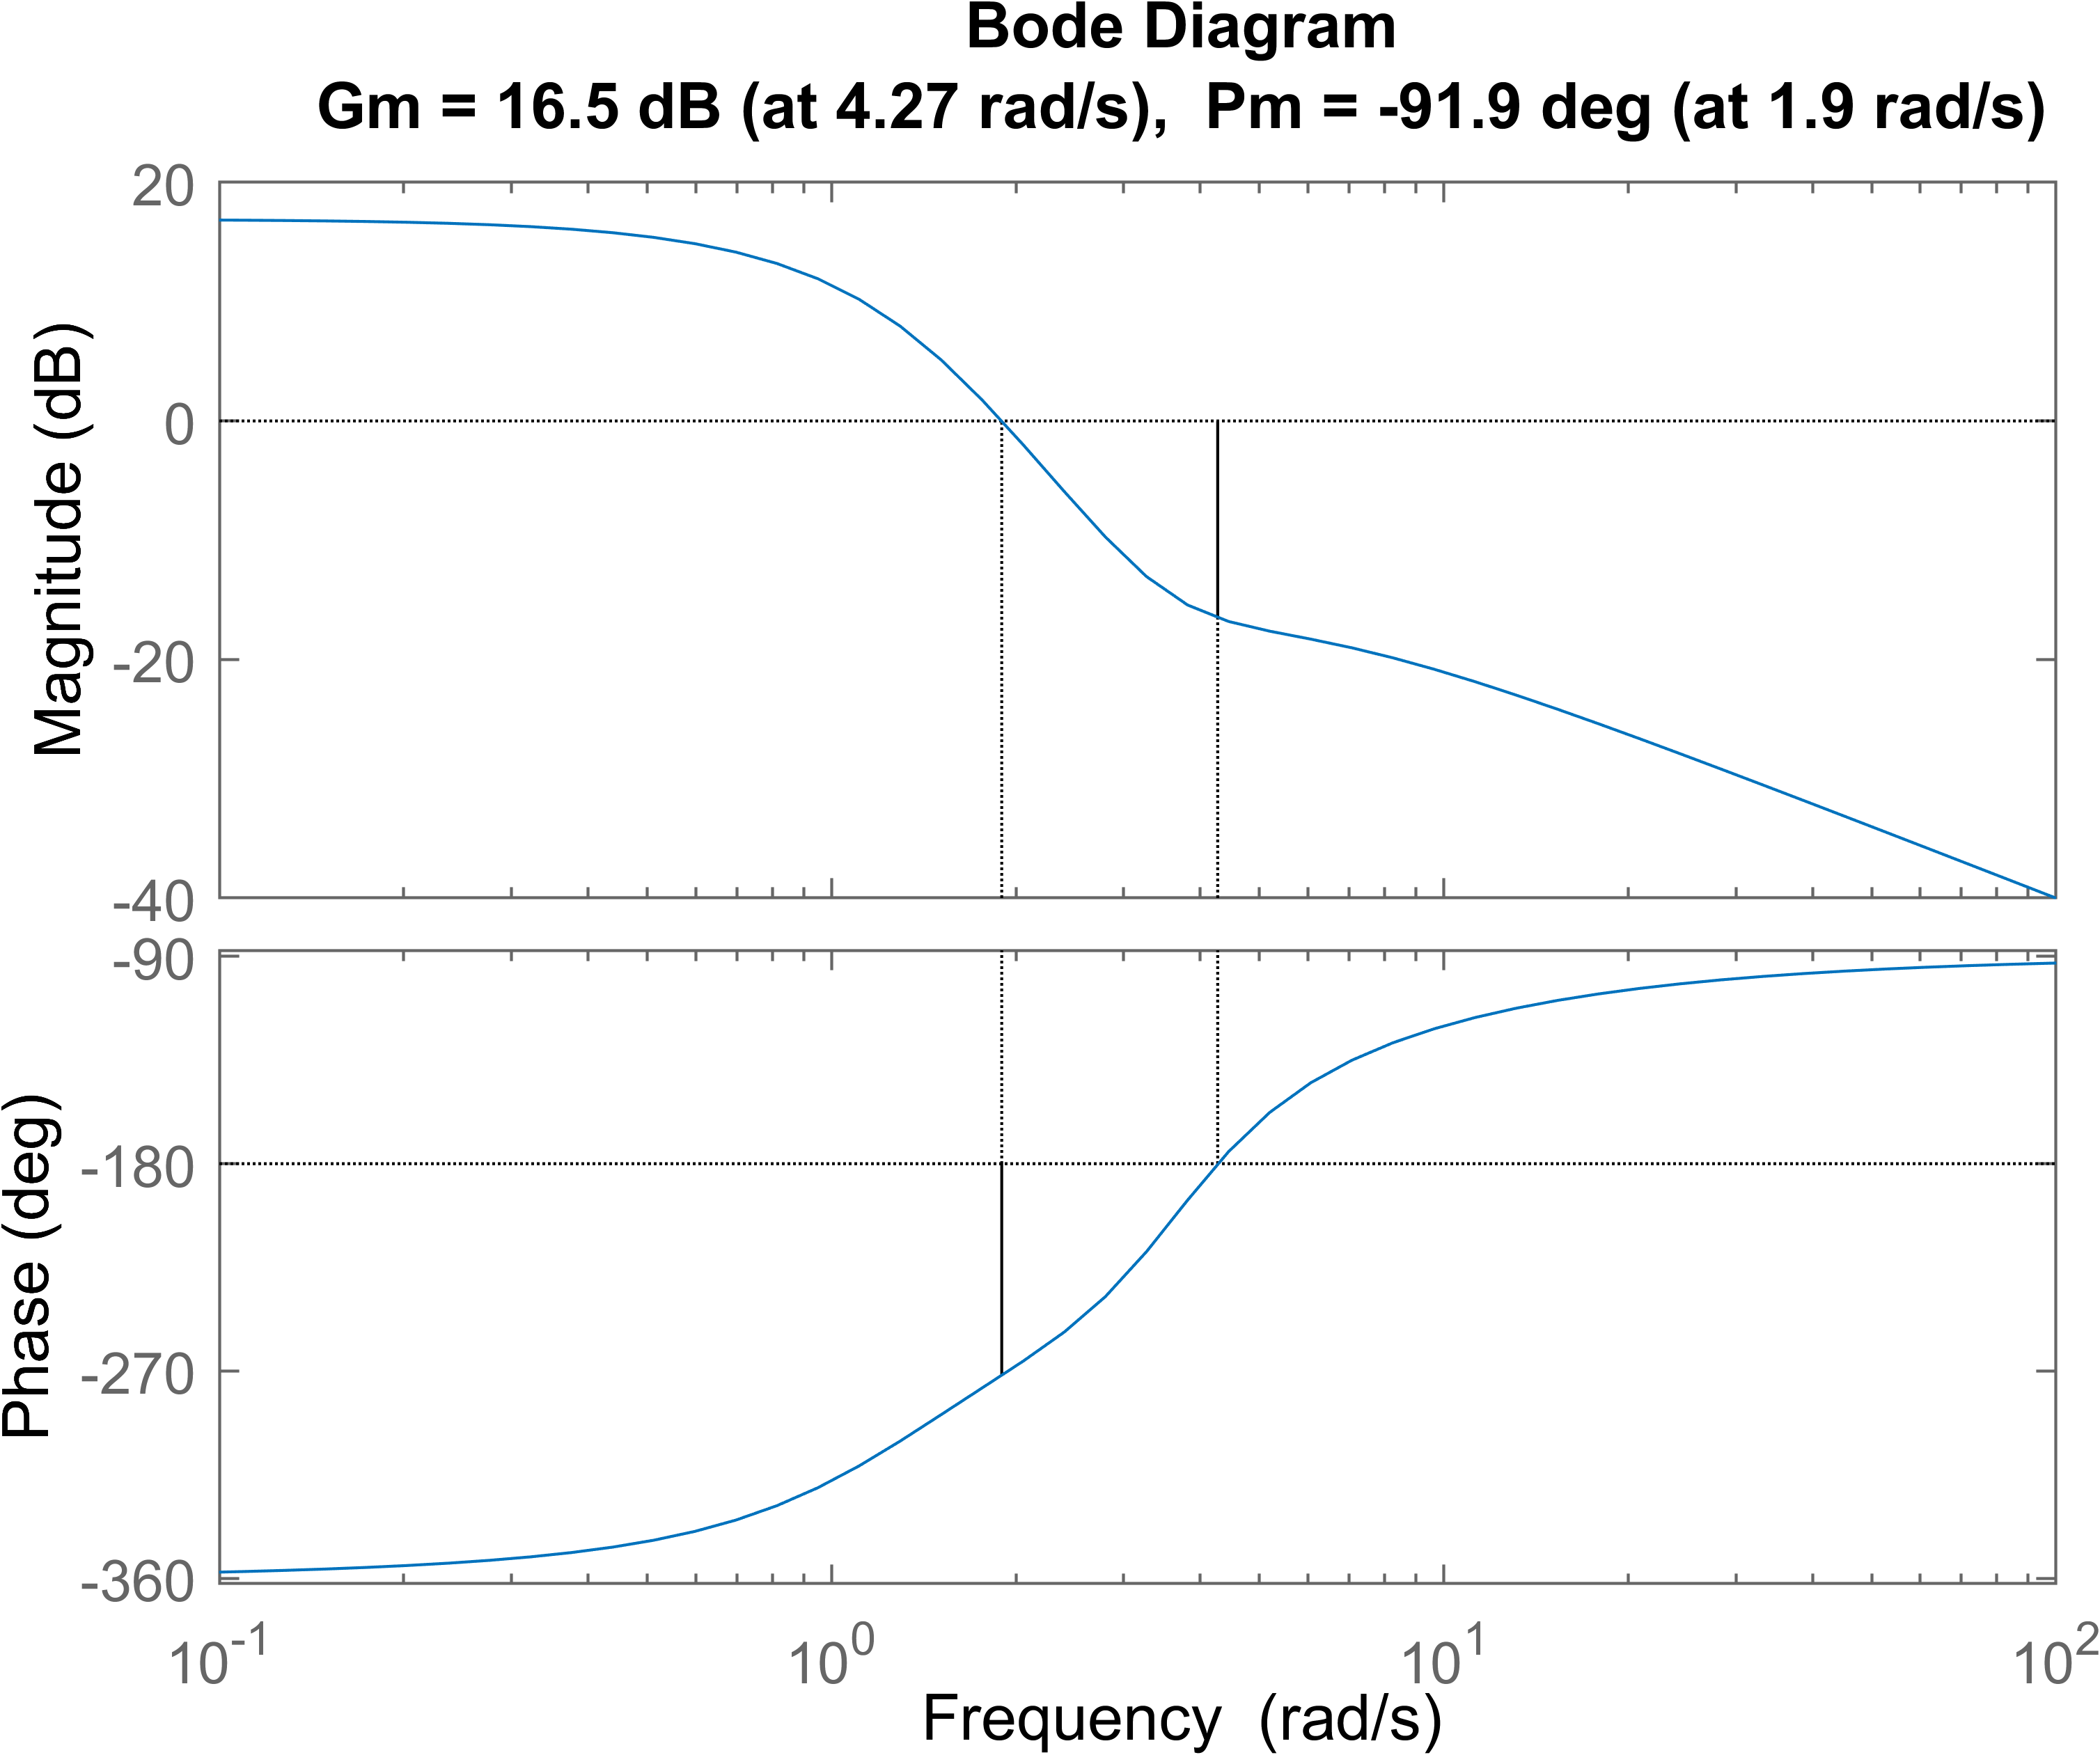
\includegraphics[width=0.7\textwidth, trim={0cm 0cm 0cm 0cm}]{../images/1_1_lapfs.png}
    \caption{ЛАФЧХ системы}
\end{figure}

ЛФЧХ не пересекает критические уровни при $L(\omega)>0$. Согласно логарифмическому критерию Найквиста замкнутая система не устойчива.

\section{Объект 2}
Вторая передаточная функция должна иметь 0 неустойчивых полюсов у разомкнутой системы и 4 неустойчивых полюса у замкнутой.
Также как и в предыдущем пункте, составим выражение для передаточной функции разомкнутой системы:
\[
Q(s) = (s+1)(s+1-i)(s+1+i)(s+2-i)(s+2+i)
\]
\[
D(s) = (s+2)(s-1-2i)(s-1+2i)(s-2-2i)(s-2+2i)
\]
\[
R(s) = D(s) - Q(s) = -11s^4 - 12^3 - 27^2 -60s +70
\]
\[
W(s) = \frac{-11s^4 - 12^3 - 27^2 -60s +70}{(s+1)(s+1-i)(s+1+i)(s+2-i)(s+2+i)}
\]

Теперь построим карту полюсов и нулей передаточной функции разомкнутой и замкнутой системы:
\begin{figure}[H]
    \centering
    \begin{minipage}{0.45\textwidth}
        \centering
        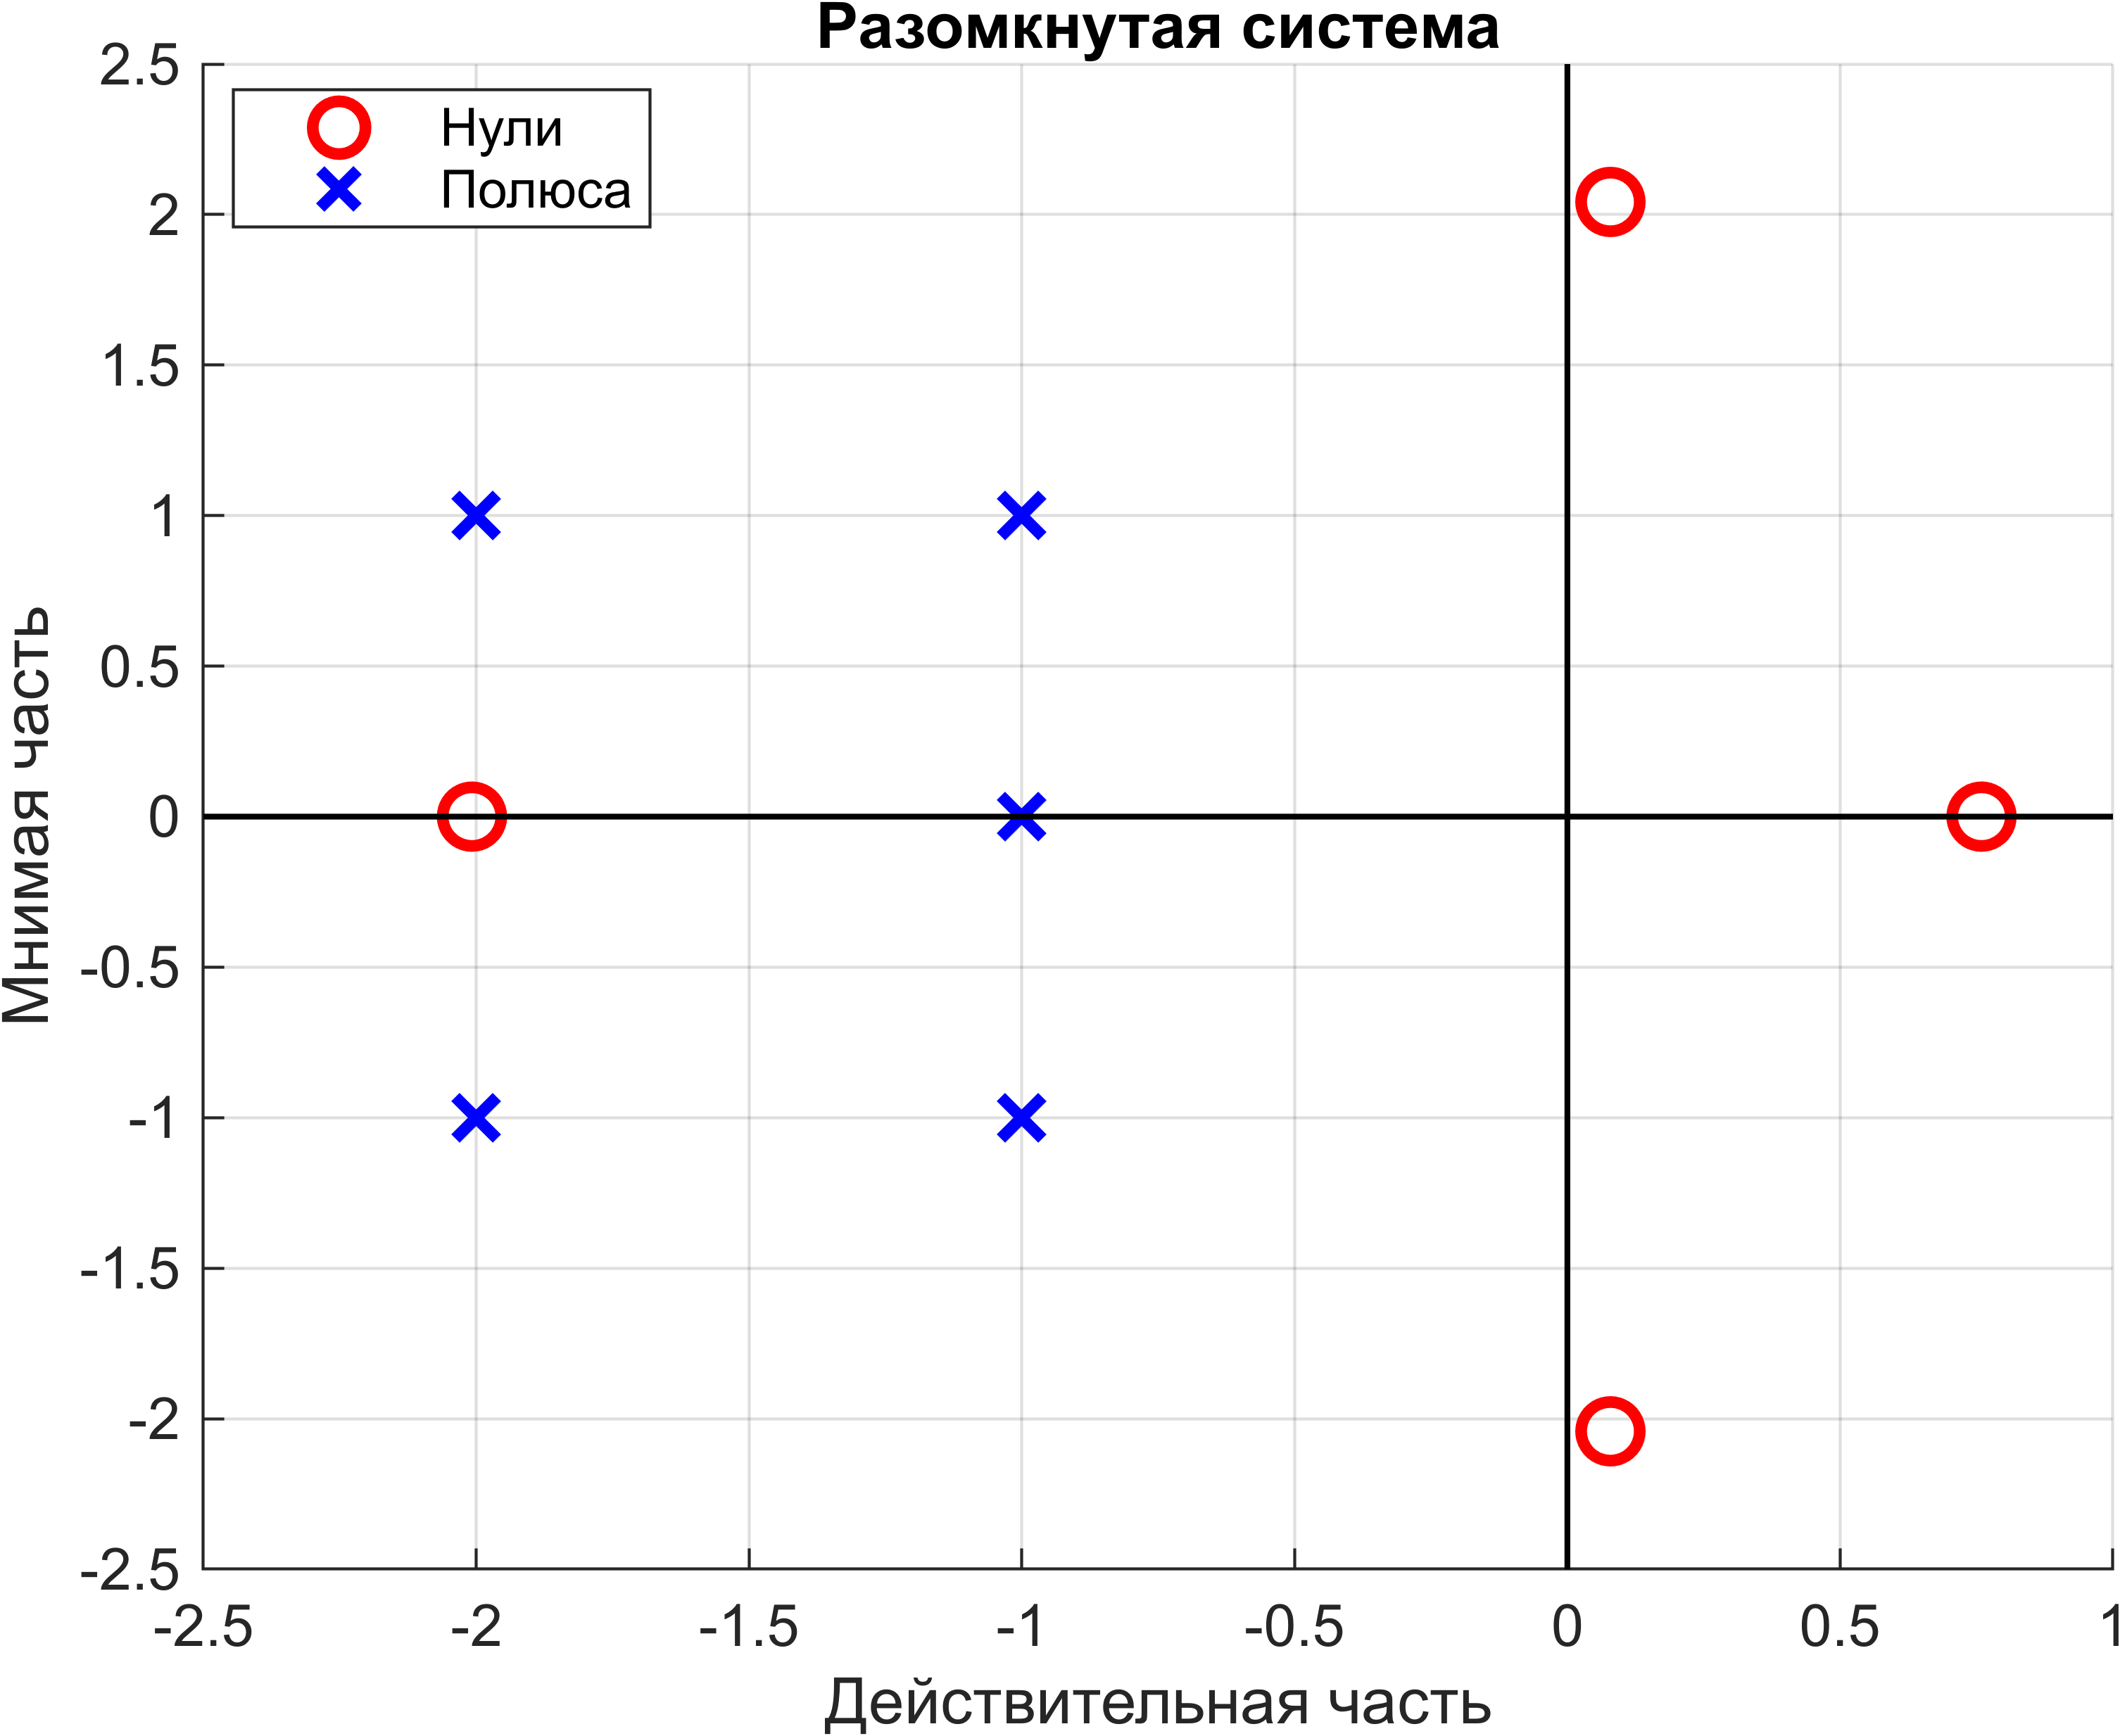
\includegraphics[width=1\textwidth, trim={0cm 0cm 0cm 0cm}]{../images/1_2_map_ol.png}
    \end{minipage}
    \hfill
    \begin{minipage}{0.45\textwidth}
        \centering
        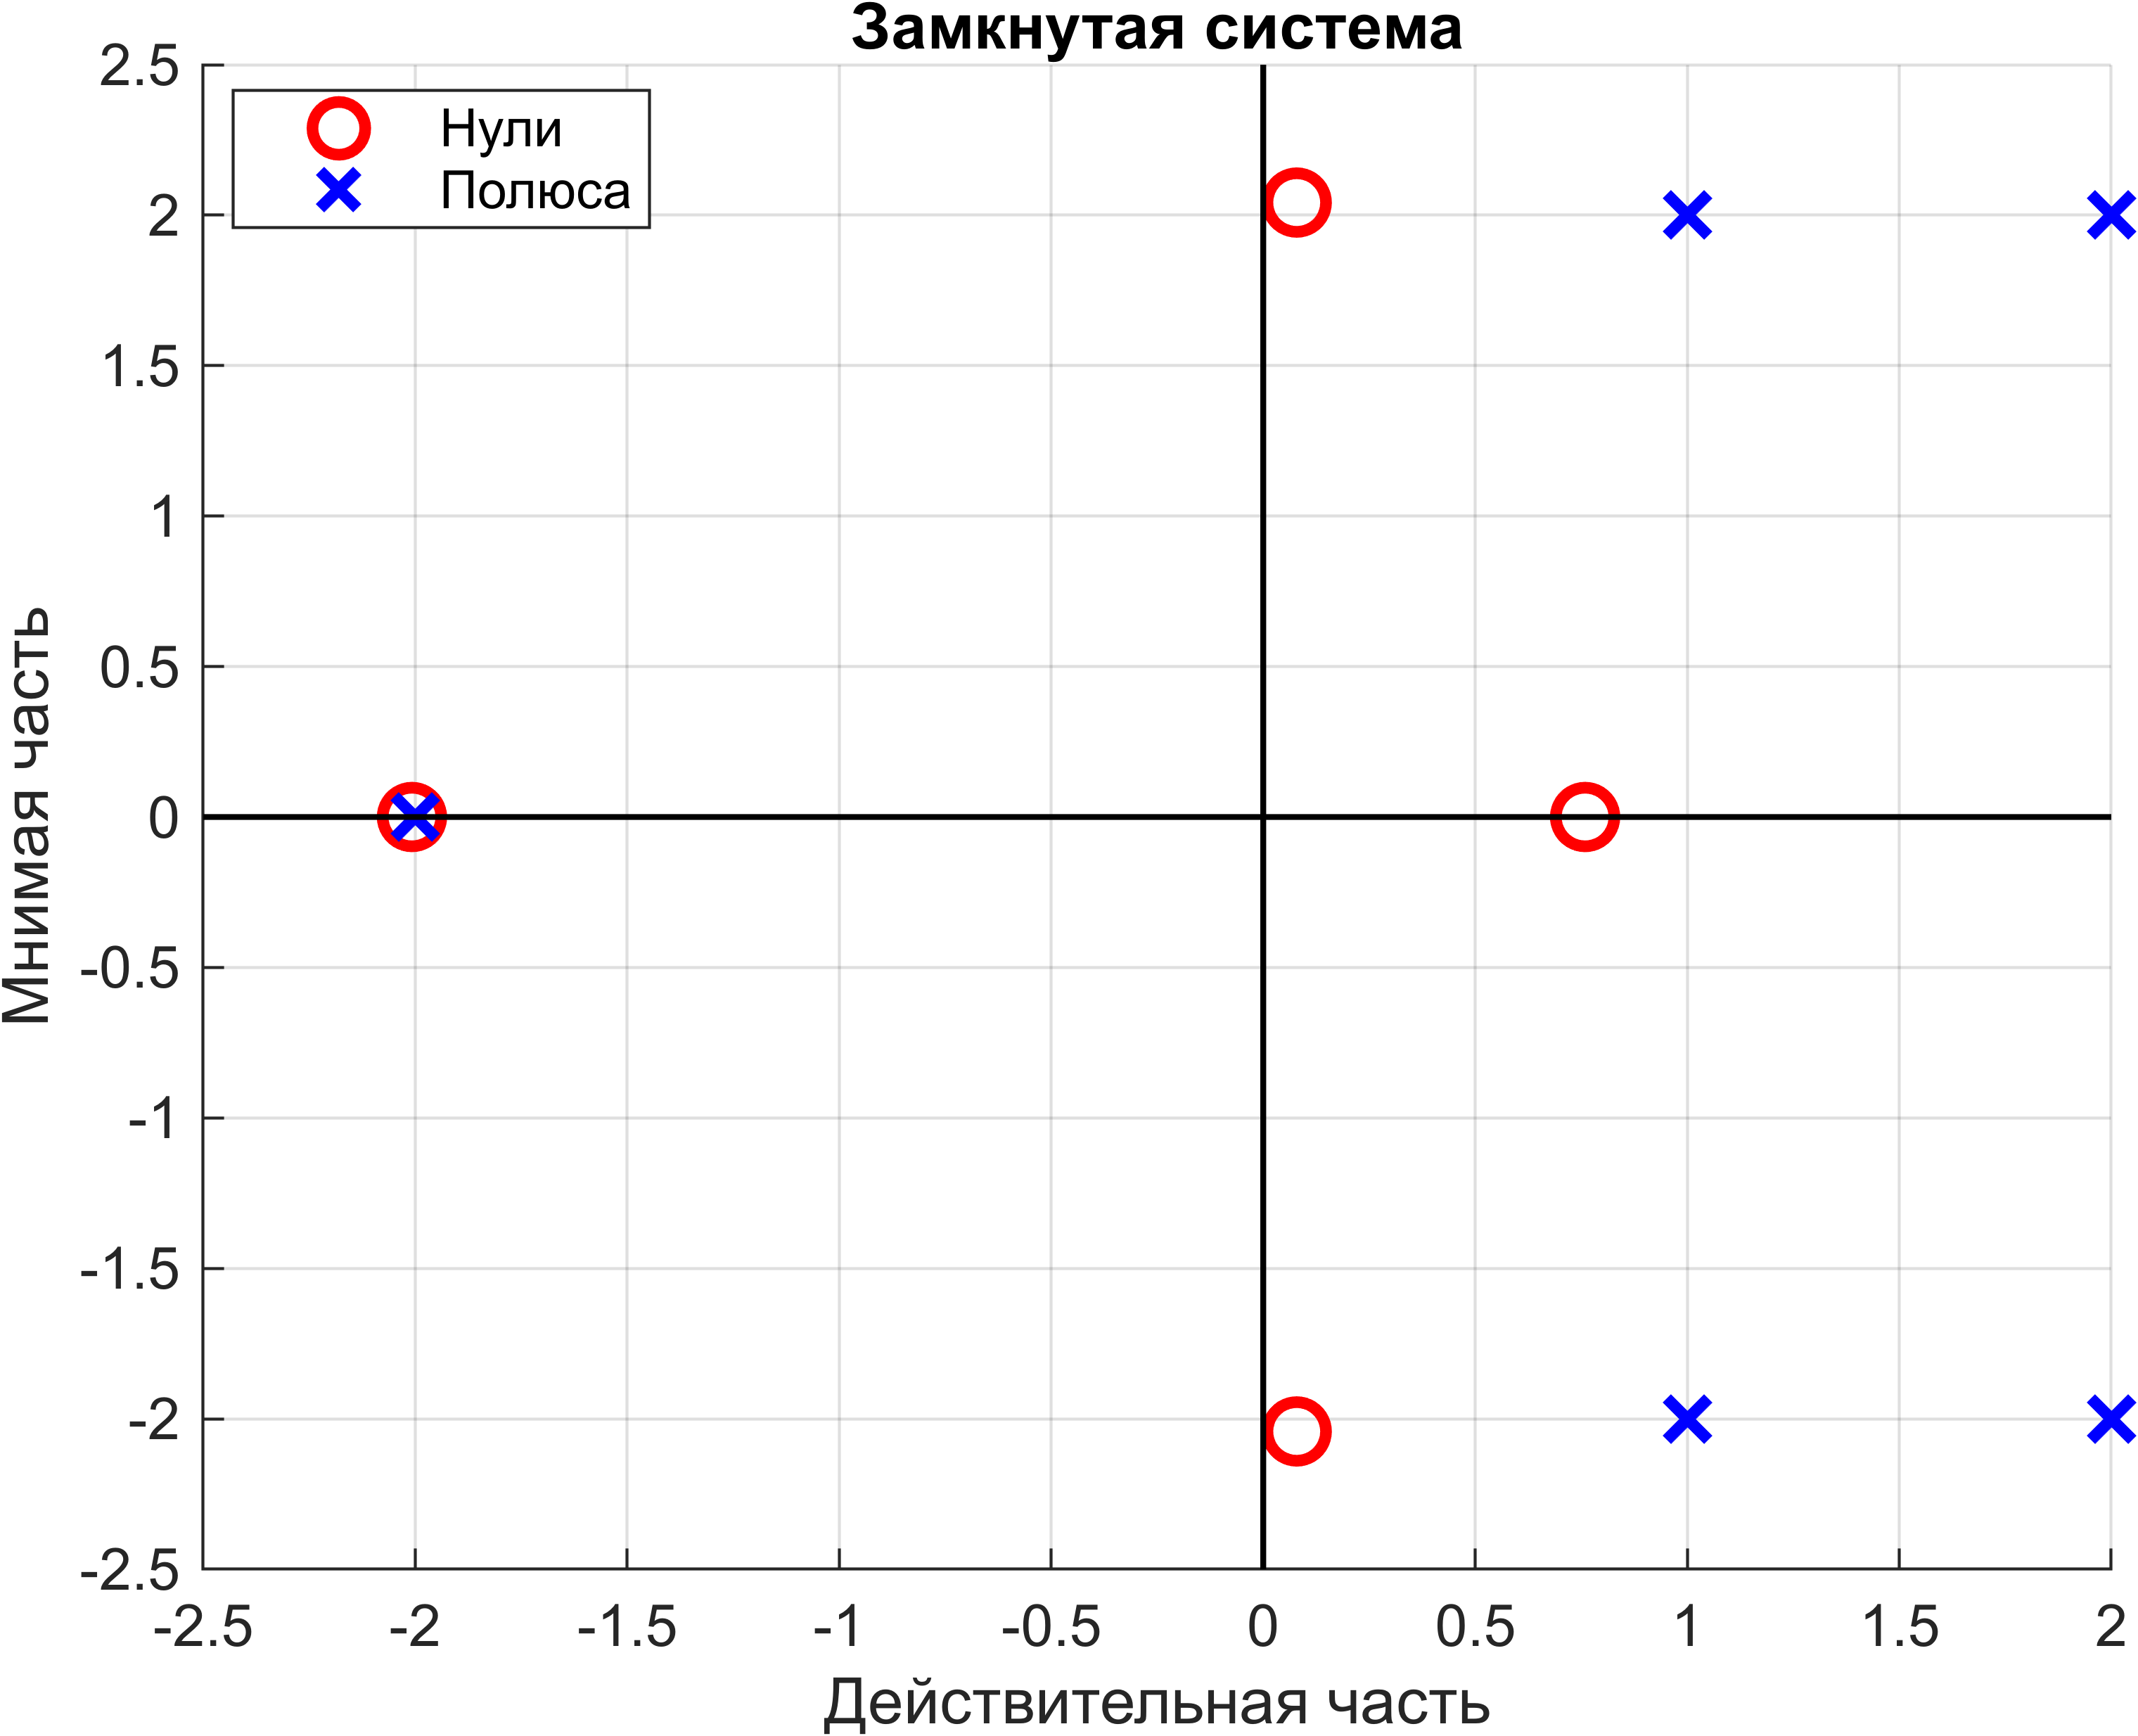
\includegraphics[width=1\textwidth, trim={0cm 0cm 0cm 0cm}]{../images/1_2_map_cl.png}
    \end{minipage}
    \caption{Карта полюсов и нулей разомкнутой и замкнутой системы}
\end{figure}

Построим переходные характеристики разомкнутой и замкнутой системы:
\begin{figure}[H]
    \centering
    \begin{minipage}{0.45\textwidth}
        \centering
        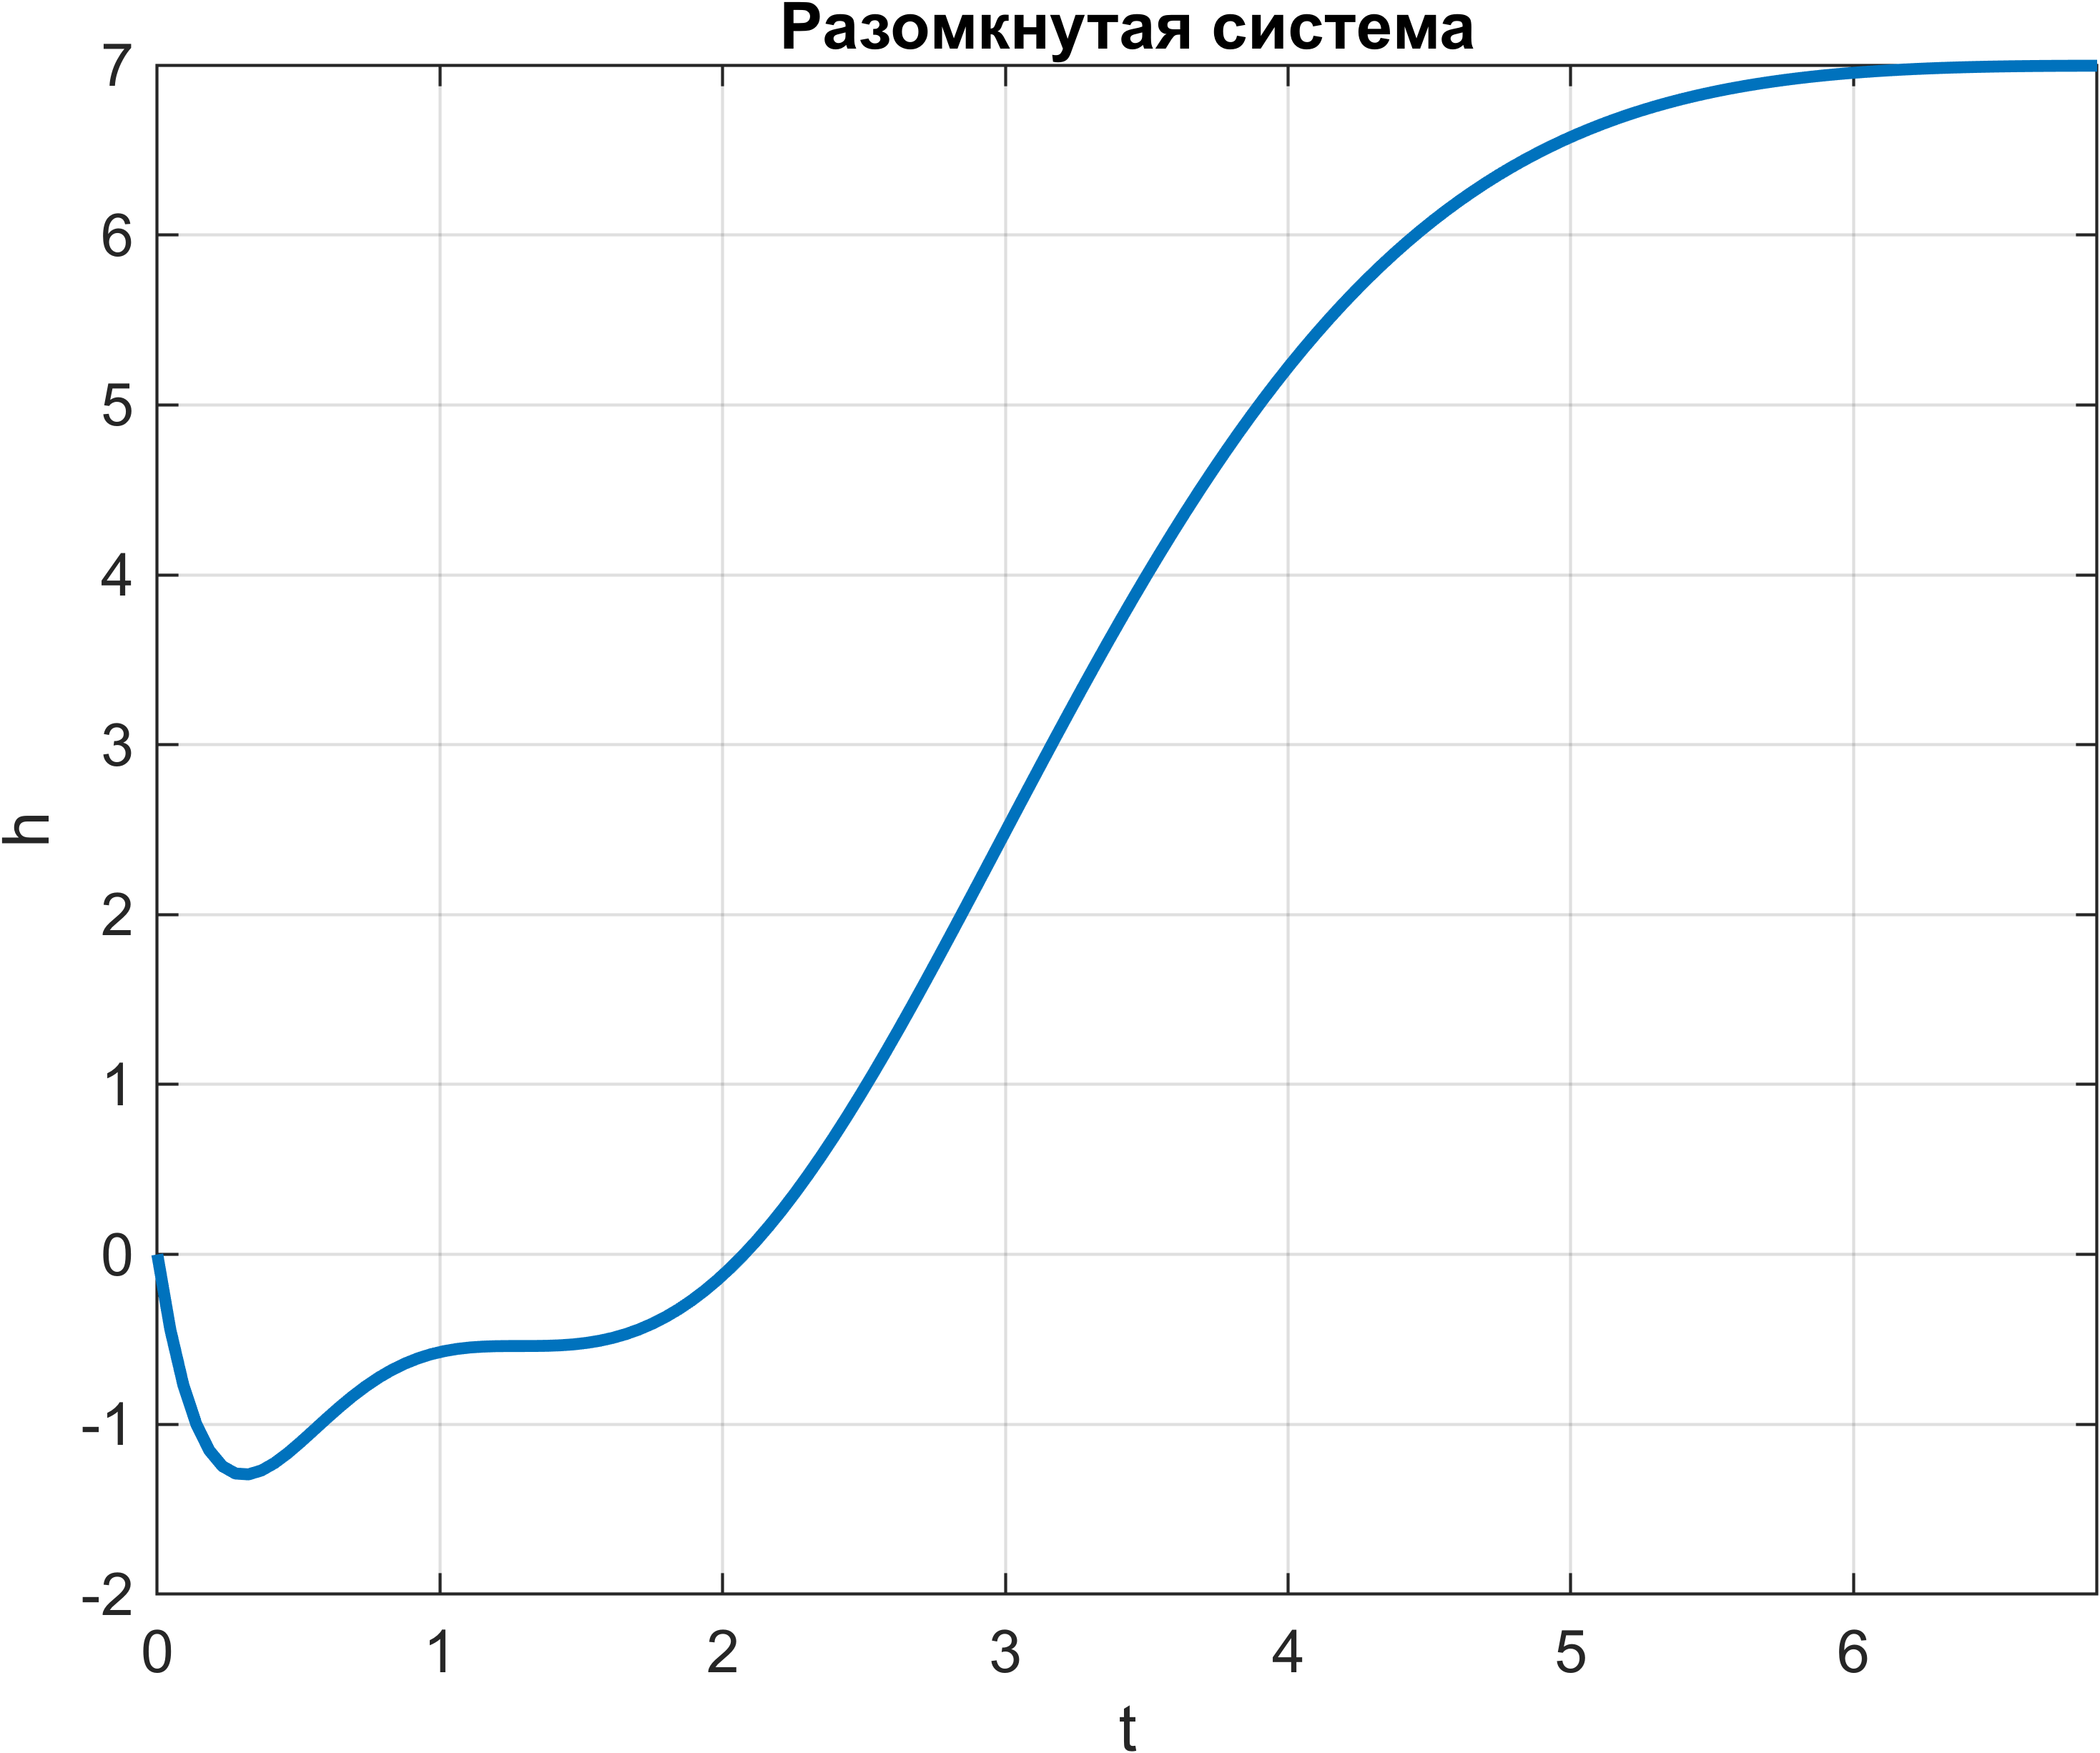
\includegraphics[width=1\textwidth, trim={0cm 0cm 0cm 0cm}]{../images/1_2_h_ol.png}
    \end{minipage}
    \hfill
    \begin{minipage}{0.45\textwidth}
        \centering
        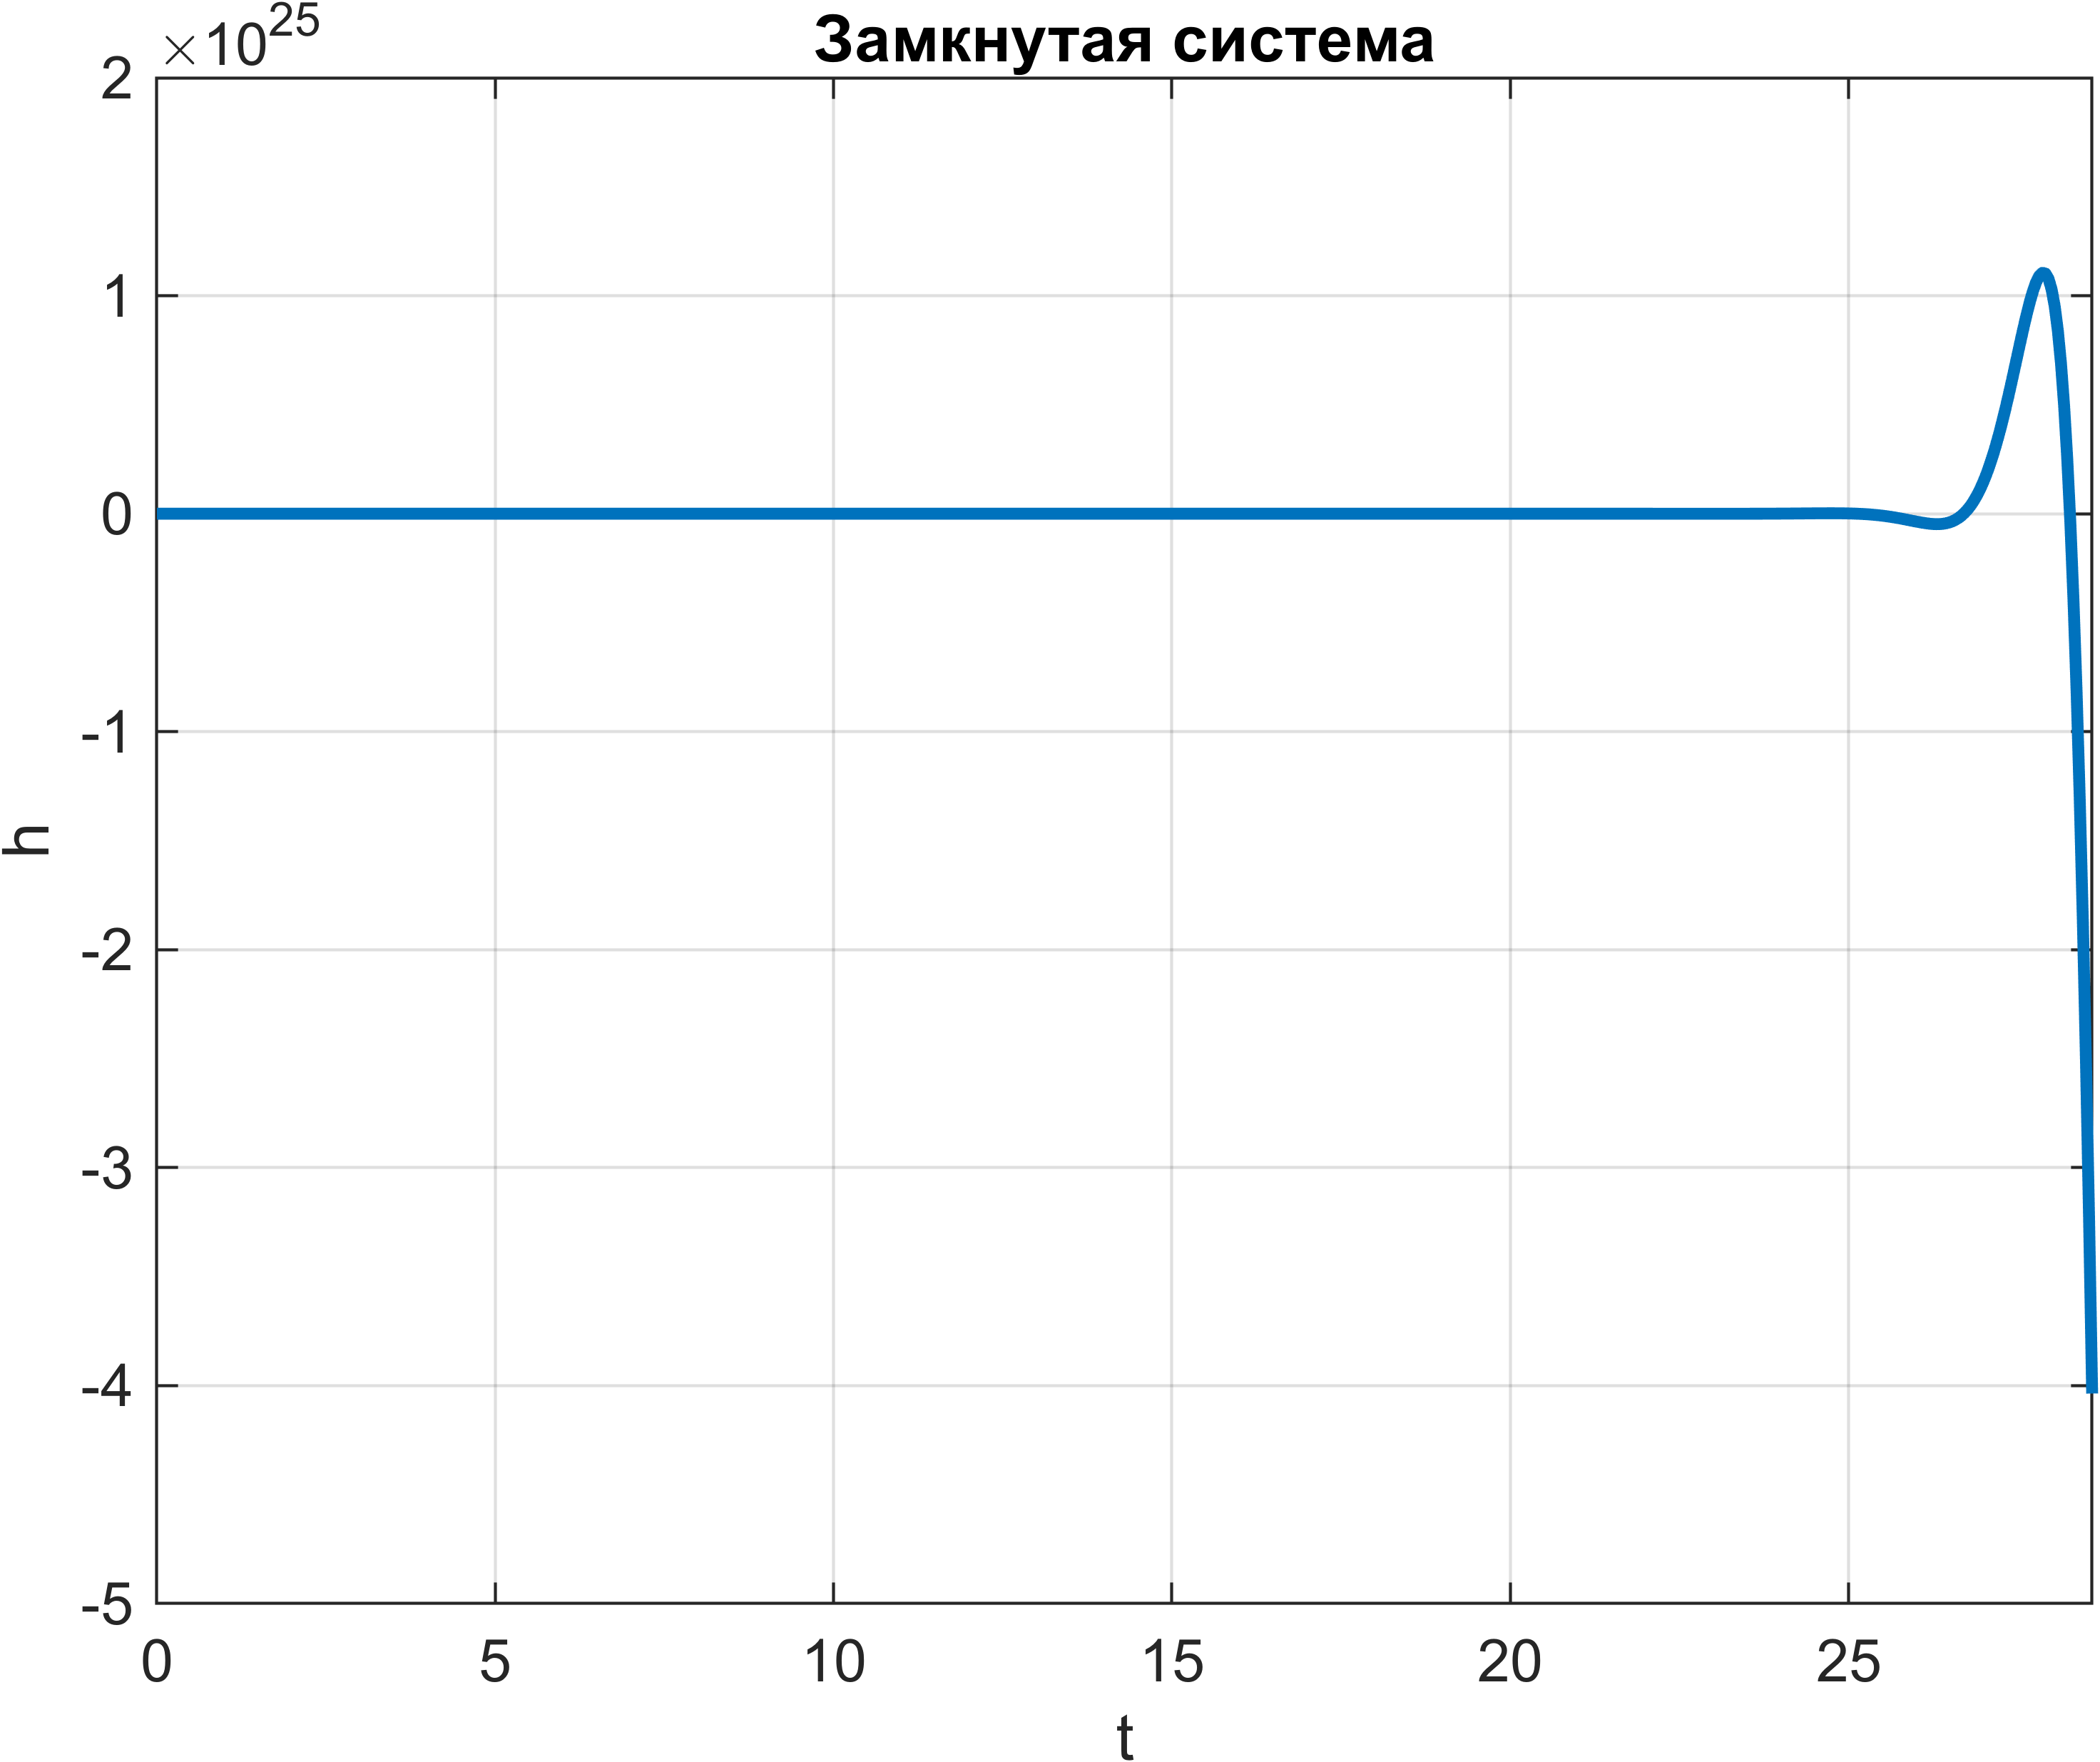
\includegraphics[width=1\textwidth, trim={0cm 0cm 0cm 0cm}]{../images/1_2_h_cl.png}
    \end{minipage}
    \caption{Переходные характеристики разомкнутой и замкнутой системы}
\end{figure}

Годограф Найквиста для данной передаточной функции:
\begin{figure}[H]
    \centering
    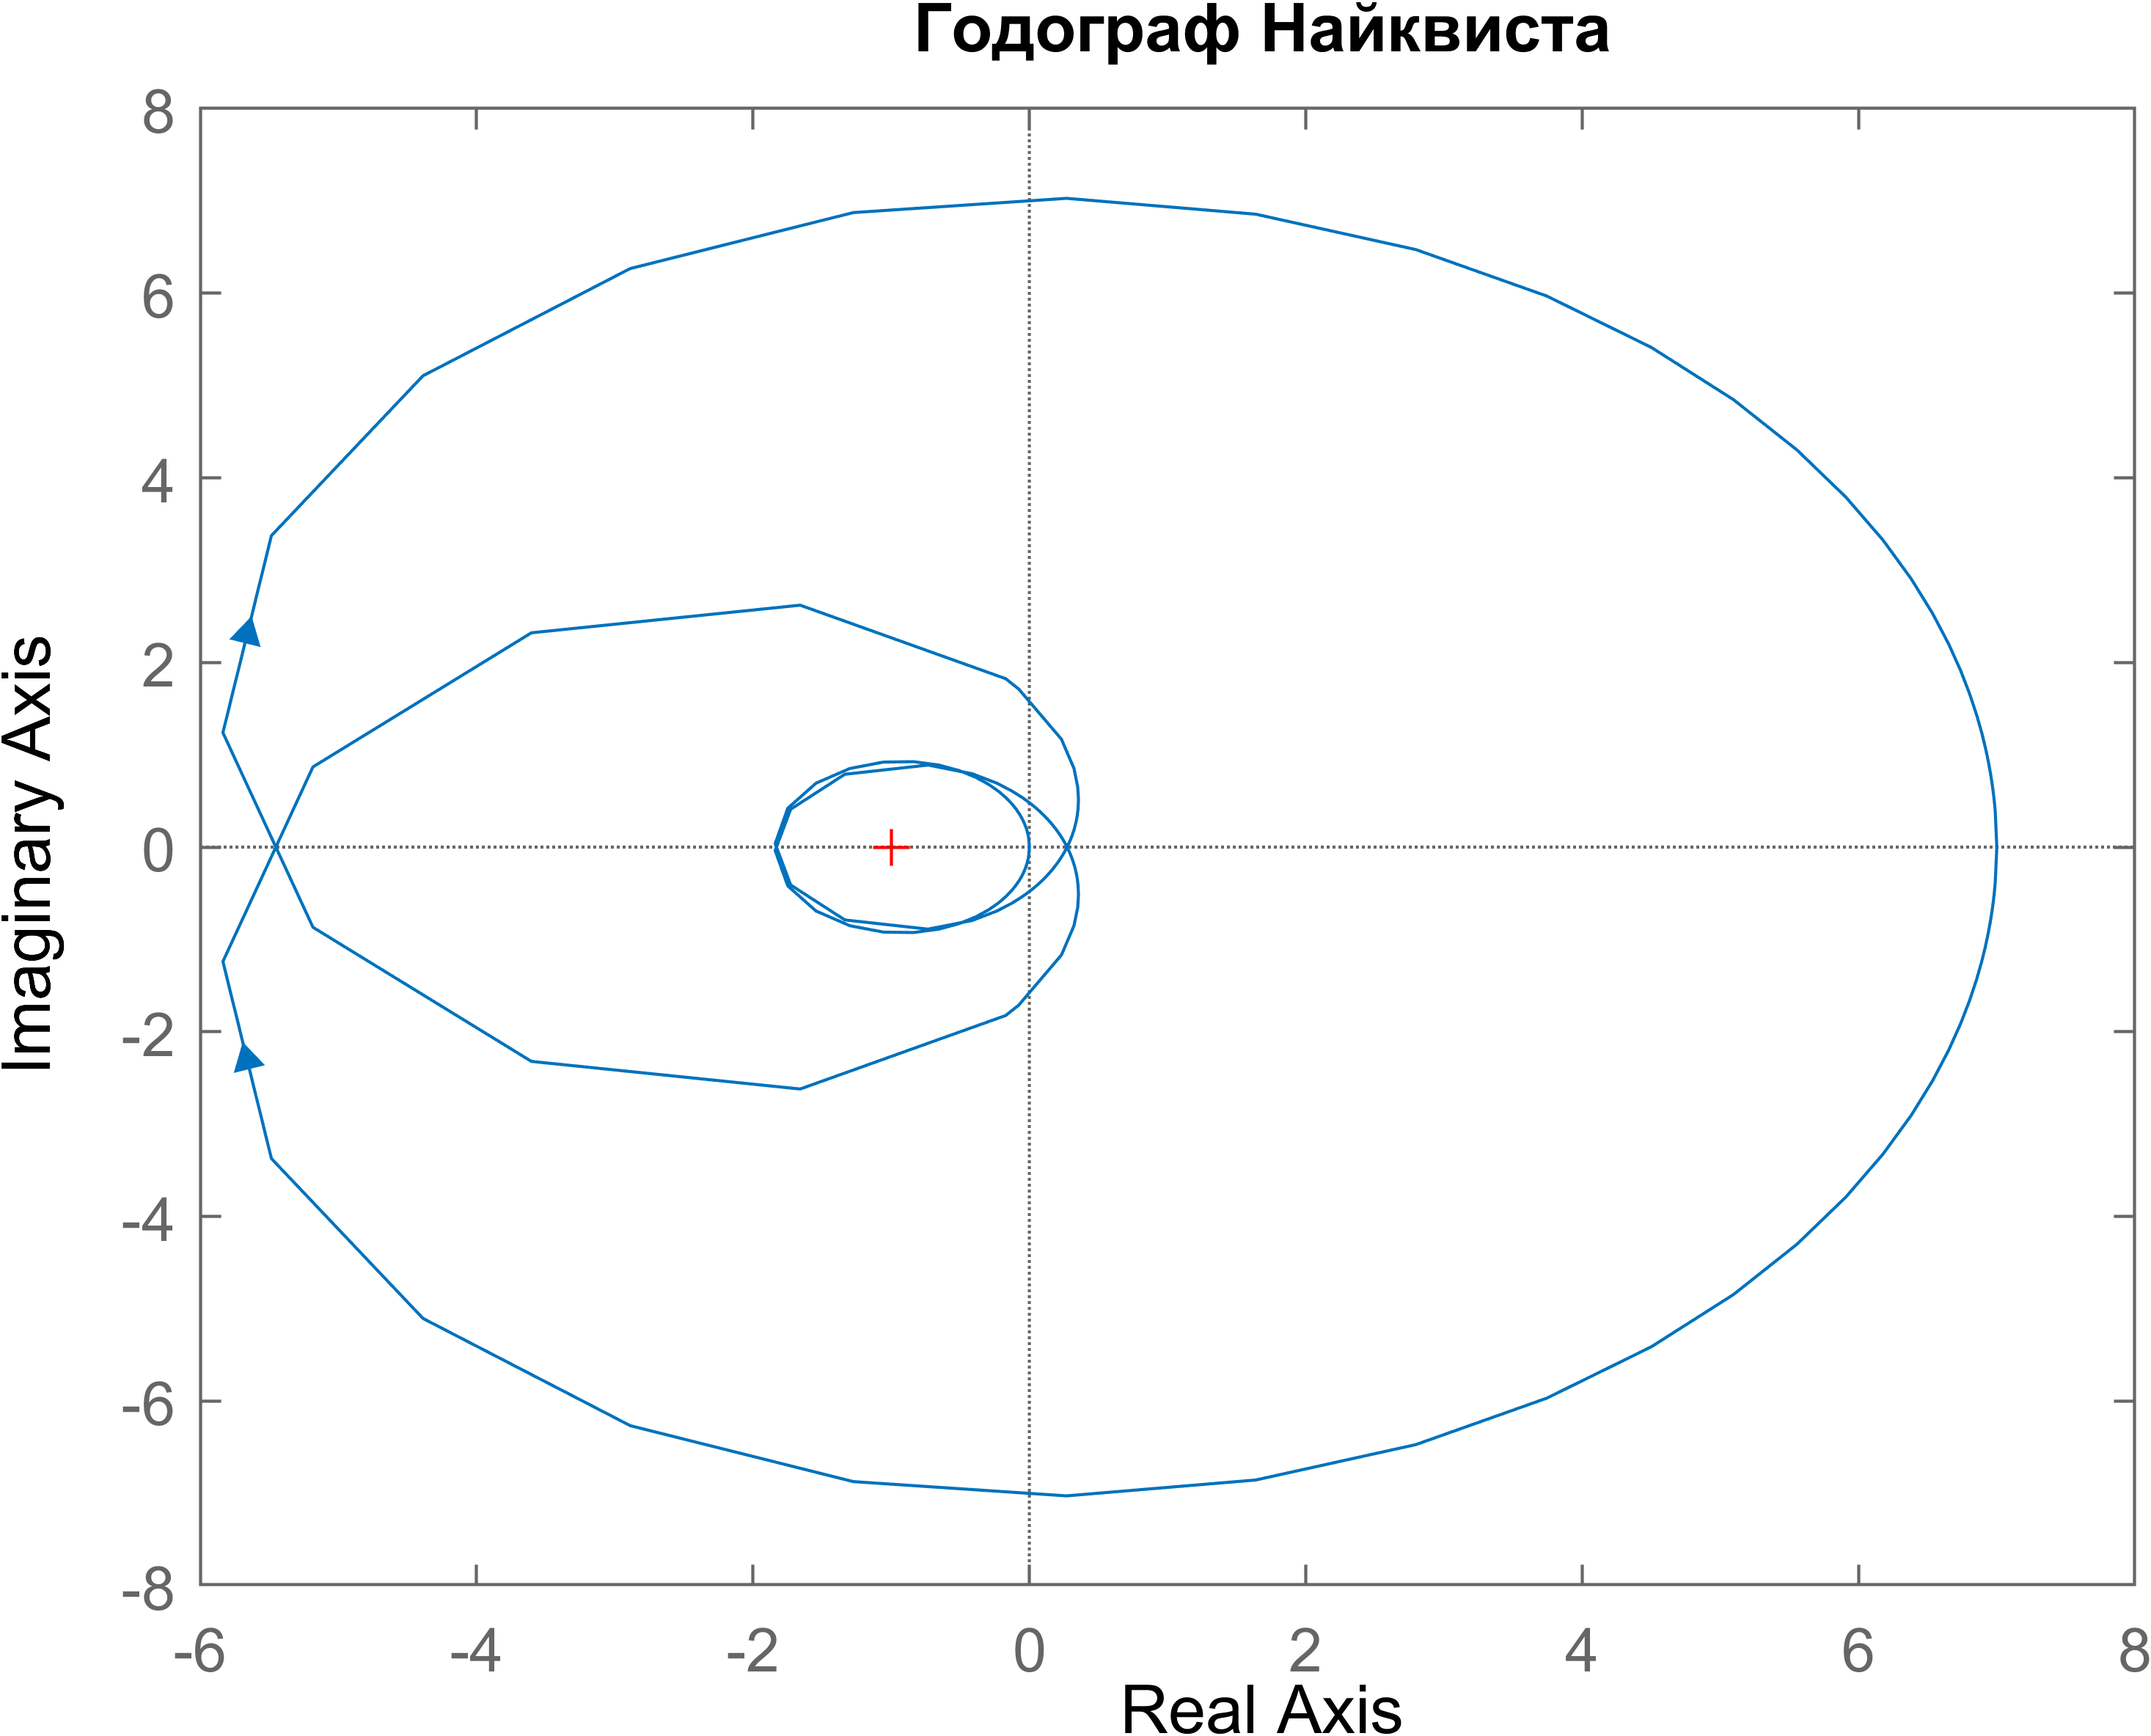
\includegraphics[width=0.7\textwidth, trim={0cm 0cm 0cm 0cm}]{../images/1_2_hod.png}
    \caption{Годограф Найквиста}
\end{figure}

Как видим, годограф совершил 4 оборота по часовой стрелке вокруг точки (-1, 0). Это соотносится с критерием Найквиста, так как
количество неустойчивых полюсов увеличилось на количество оборотов годографа при замыкании системы.

Рассмотрим ЛАФЧХ для данной передаточной функции:
\begin{figure}[H]
    \centering
    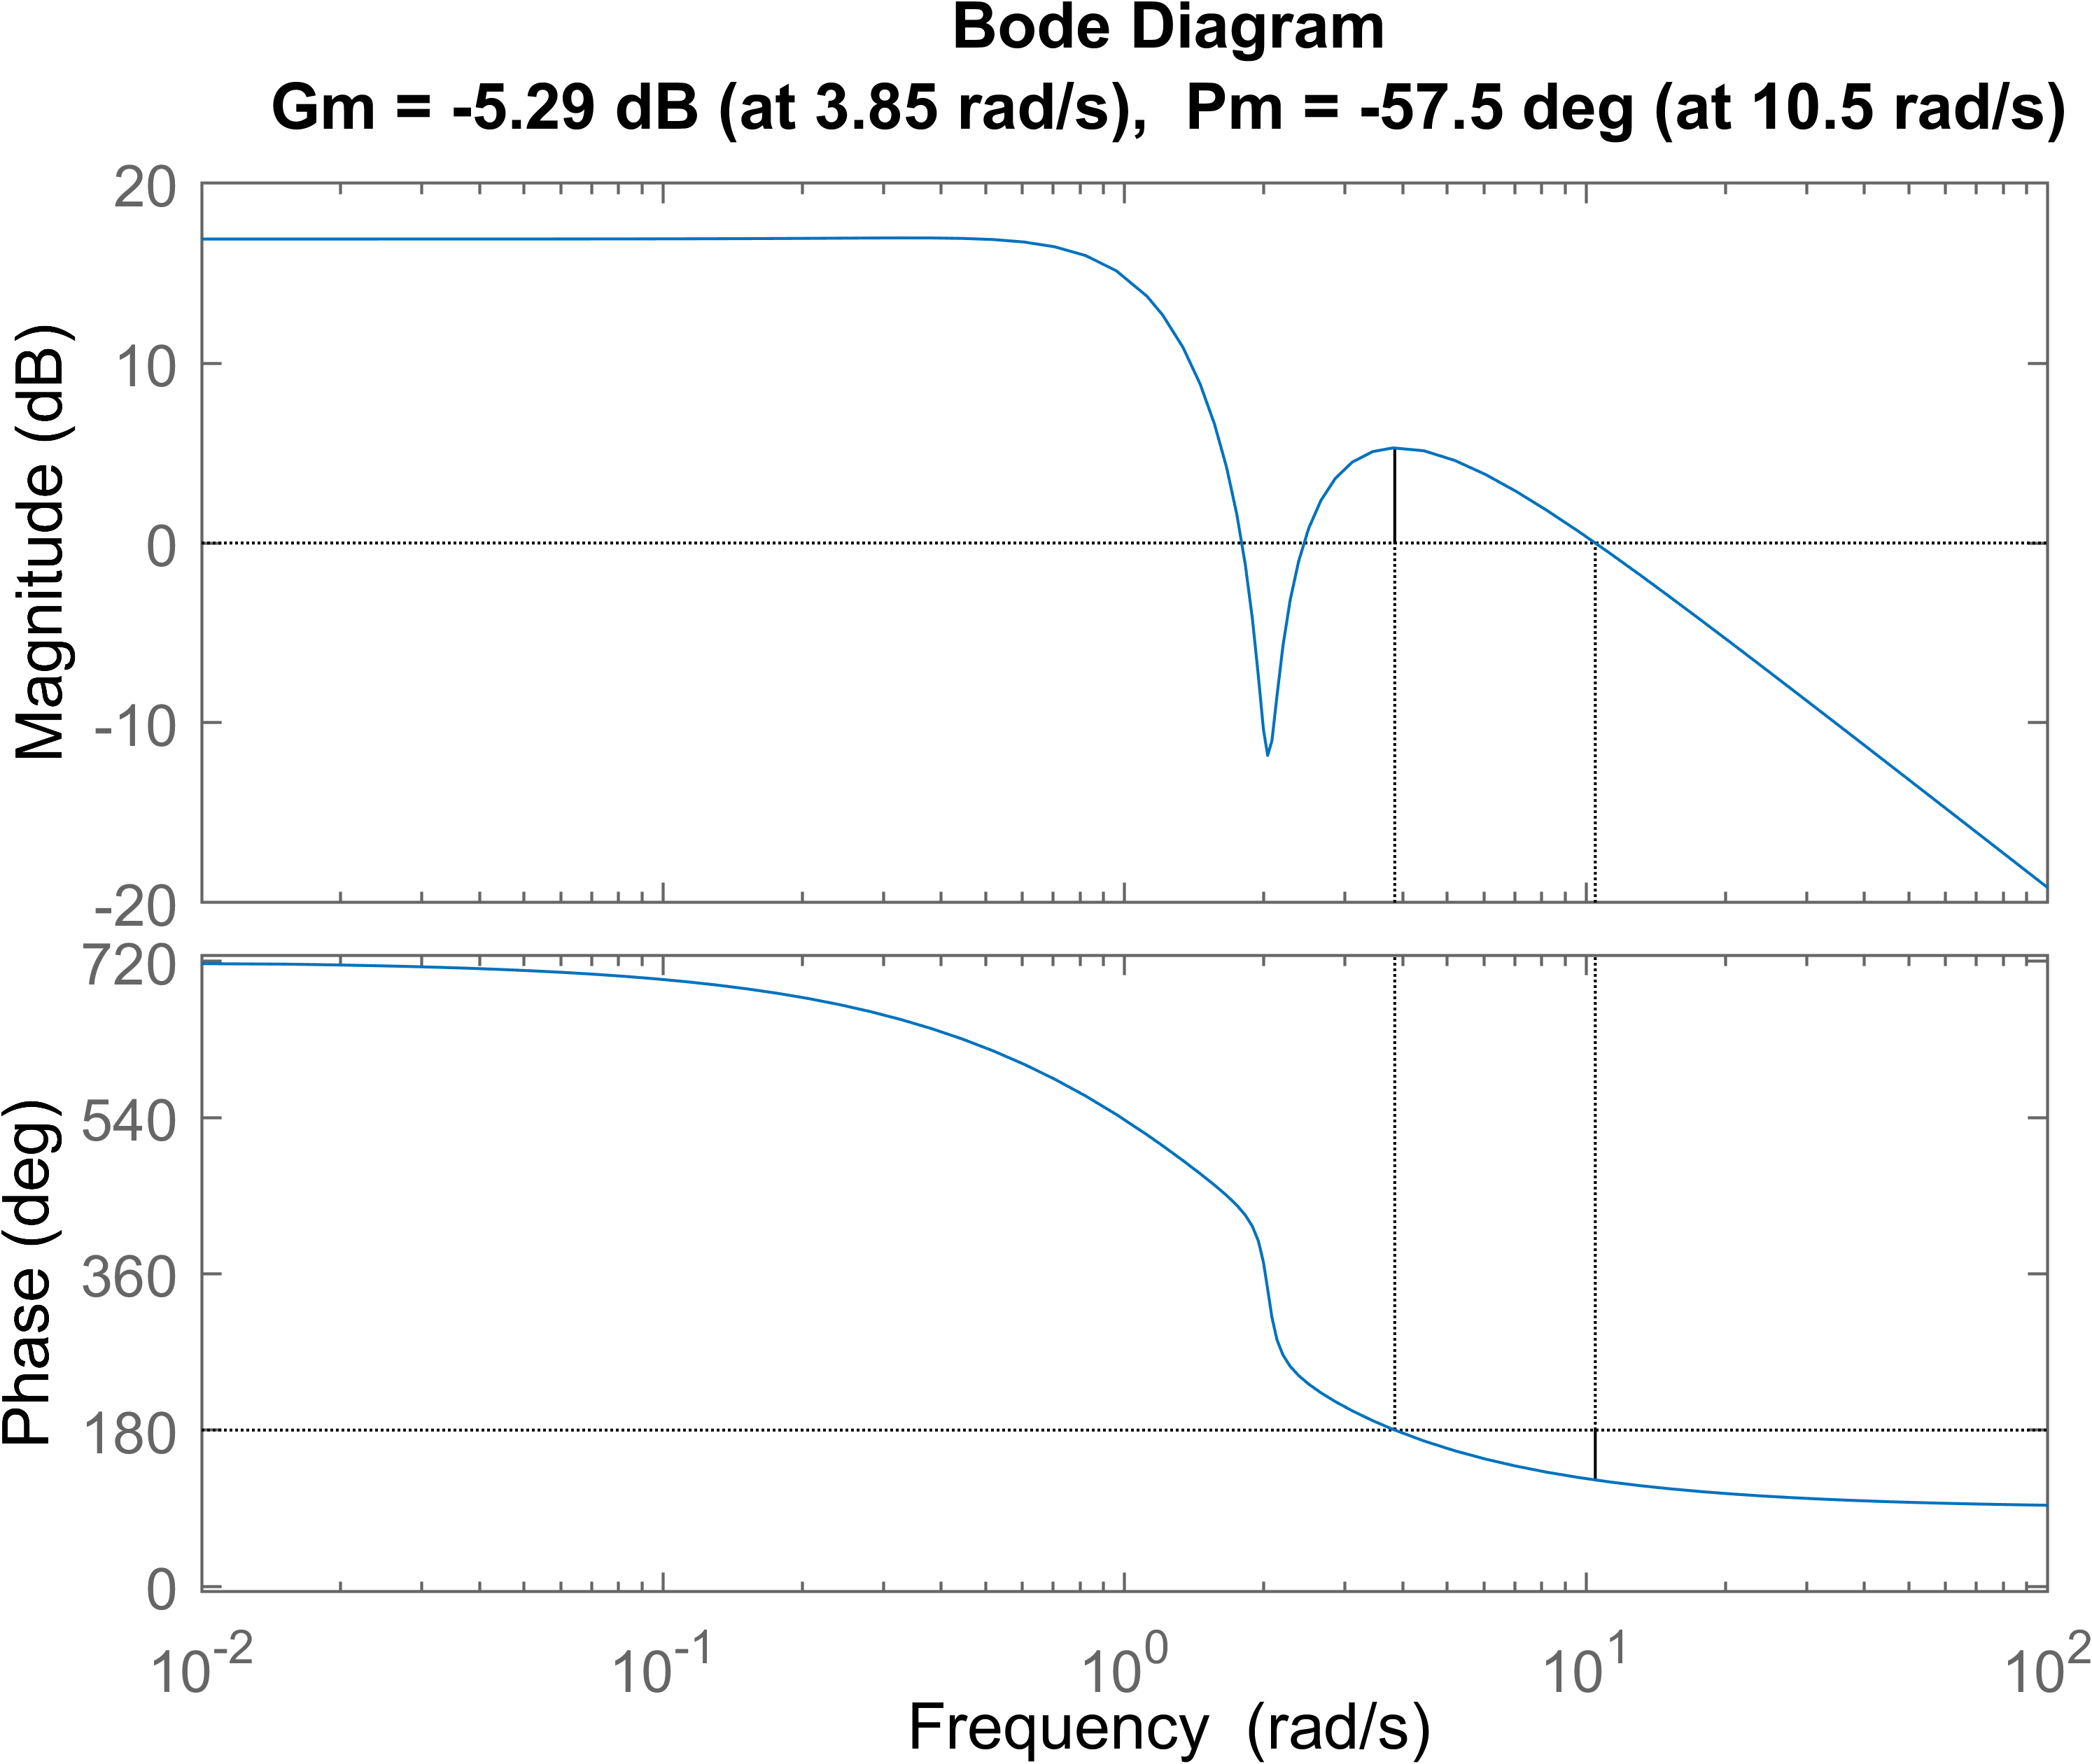
\includegraphics[width=0.7\textwidth, trim={0cm 0cm 0cm 0cm}]{../images/1_2_lapfs.png}
    \caption{ЛАФЧХ системы}
\end{figure}

Видно, что частота среза находится больше критической частоты, что соответствует неустойчивости системы.

\section{Объект 3}
Третья передаточная функция должна иметь 4 устойчивых полюса у разомкнутой системы и 0 устойчивых полюсов у замкнутой.
Также как и в предыдущих пунктах, составим выражение для передаточной функции разомкнутой системы:
\[
Q(s) = (s+1)(s-1-i)(s-1+i)(s-2-i)(s-2+i)
\]
\[
D(s) = (s+2)(s+1-2i)(s+1+2i)(s+2-2i)(s+2+2i)
\]
\[
R(s) = D(s) - Q(s) = 13s^4 + 18s^3 + 51s^2 - 54s + 10
\]
\[
W(s) = \frac{13s^4 + 18s^3 + 51s^2 - 54s + 10}{(s+1)(s-1-i)(s-1+i)(s-2-i)(s-2+i)}
\]

Теперь построим карту полюсов и нулей передаточной функции разомкнутой и замкнутой системы:
\begin{figure}[H]
    \centering
    \begin{minipage}{0.45\textwidth}
        \centering
        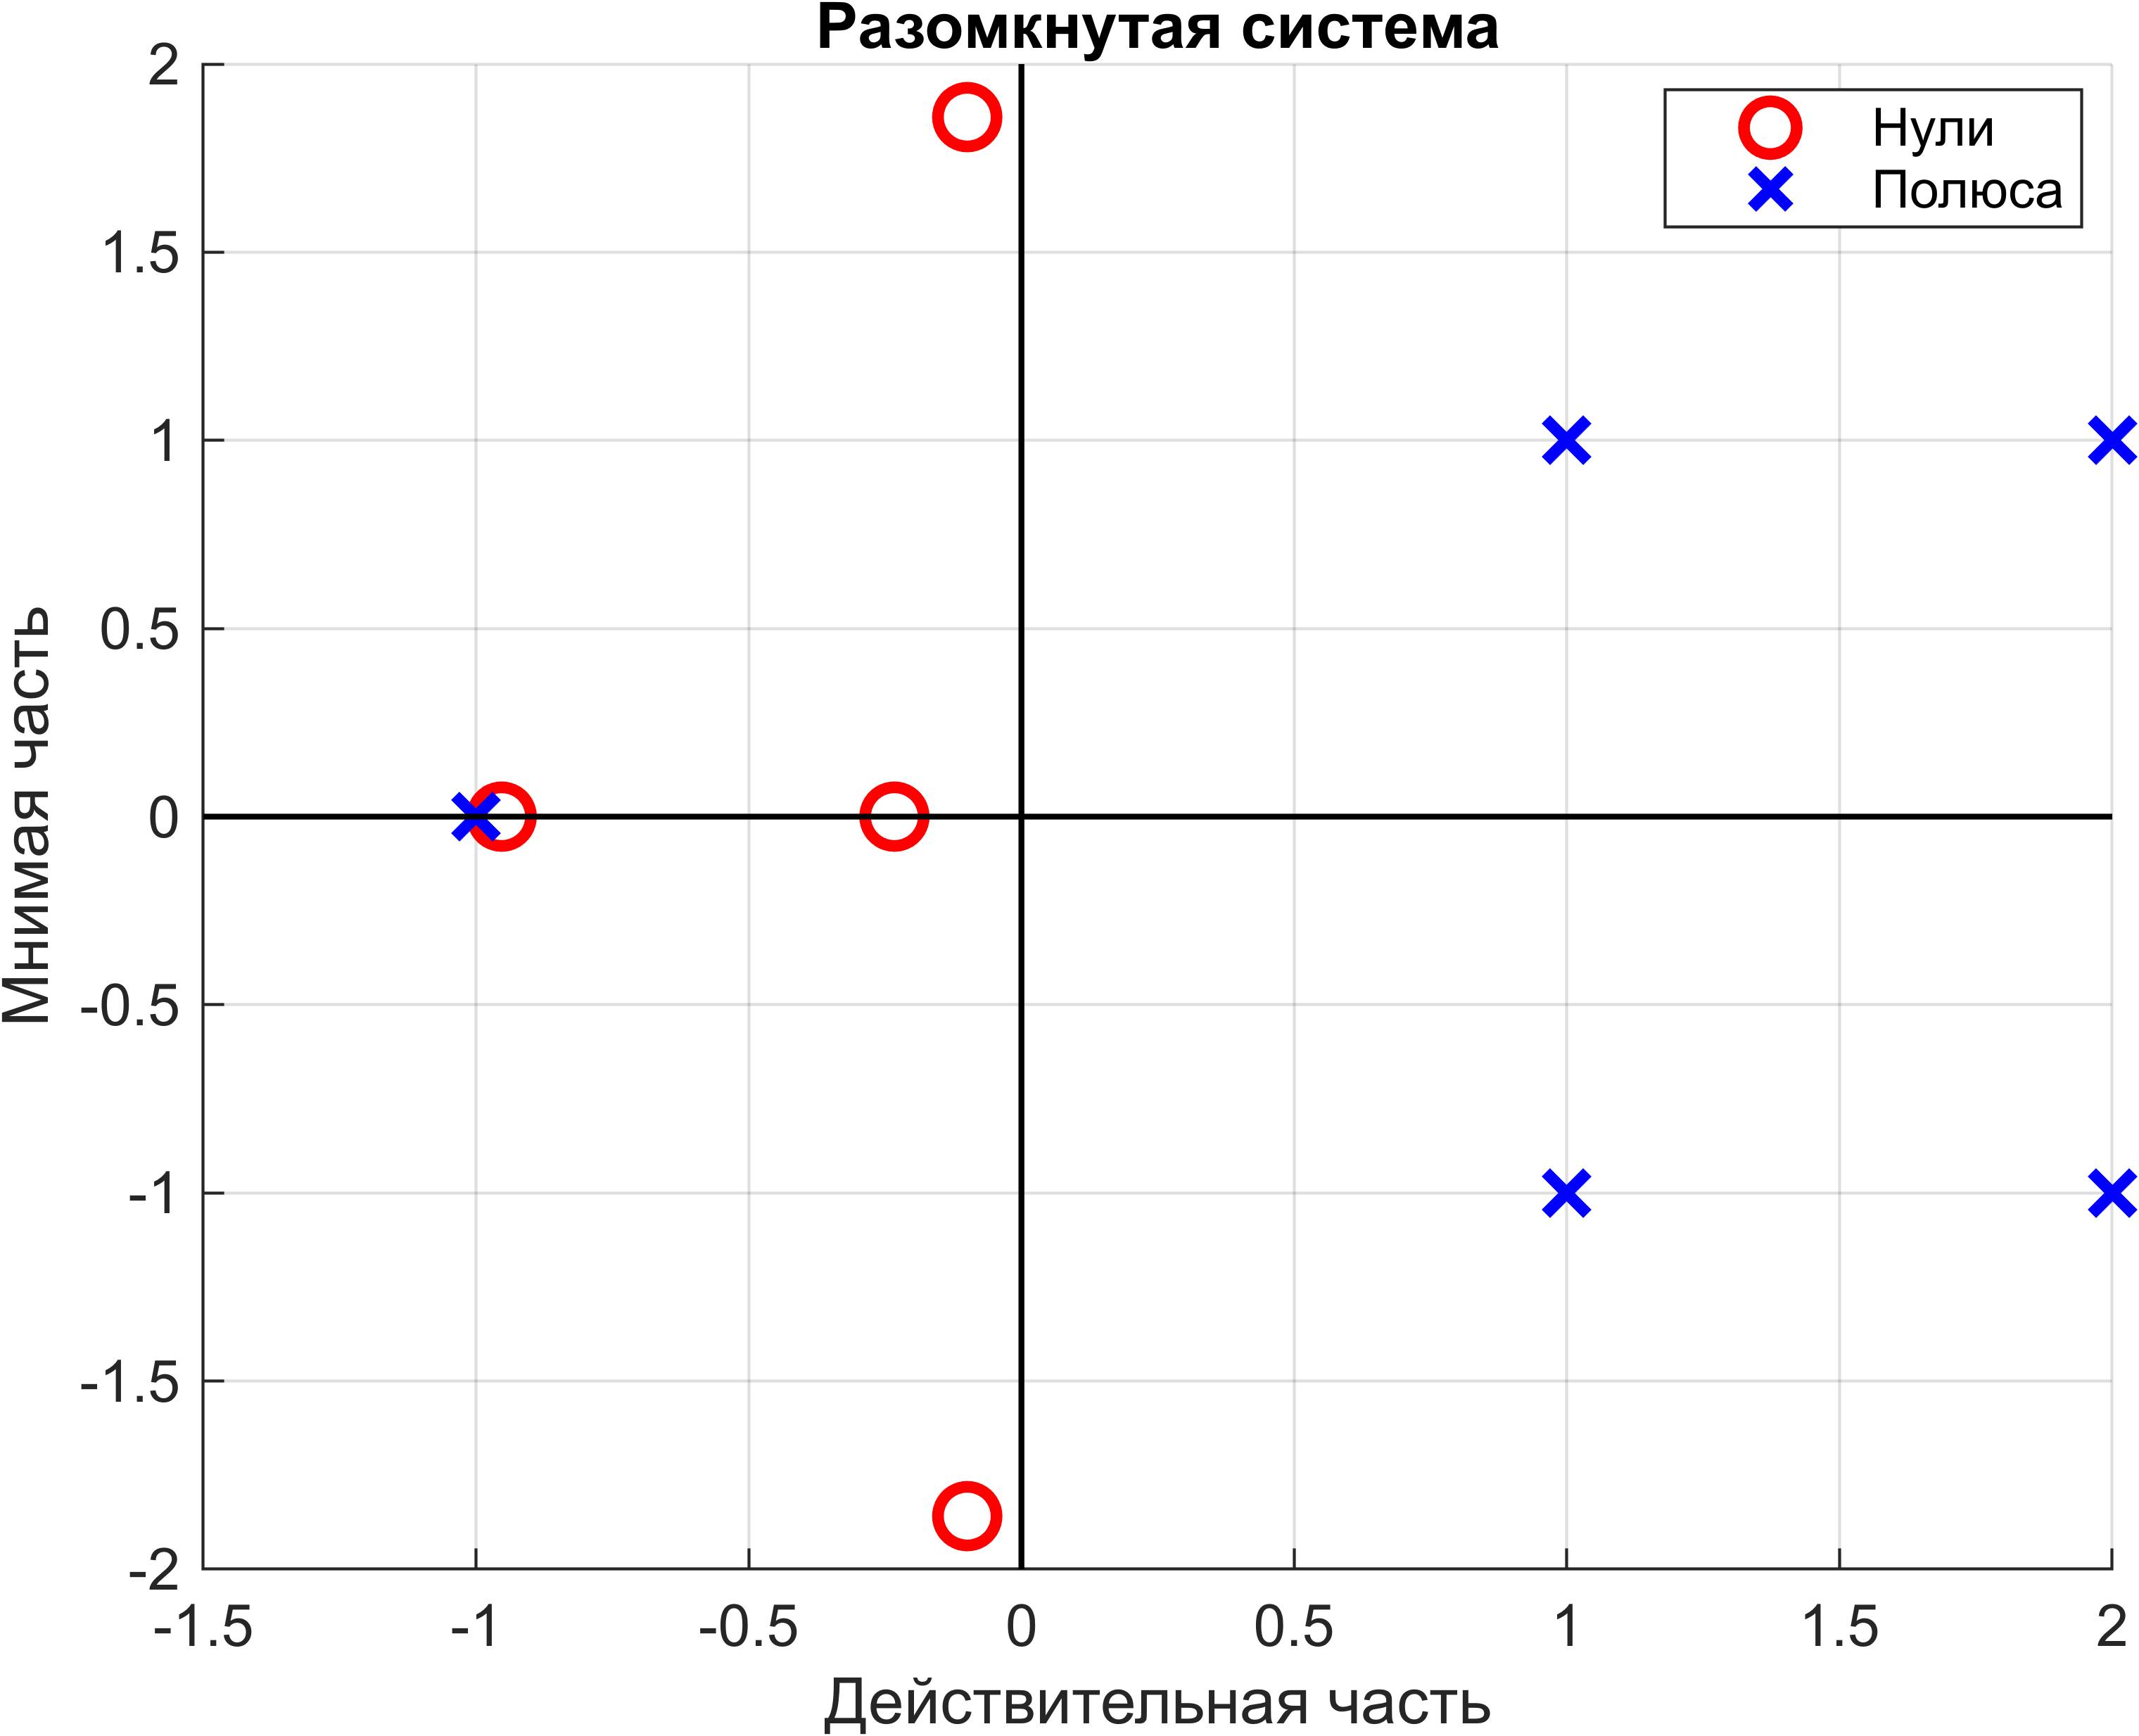
\includegraphics[width=1\textwidth, trim={0cm 0cm 0cm 0cm}]{../images/1_3_map_ol.png}
    \end{minipage}
    \hfill
    \begin{minipage}{0.45\textwidth}
        \centering
        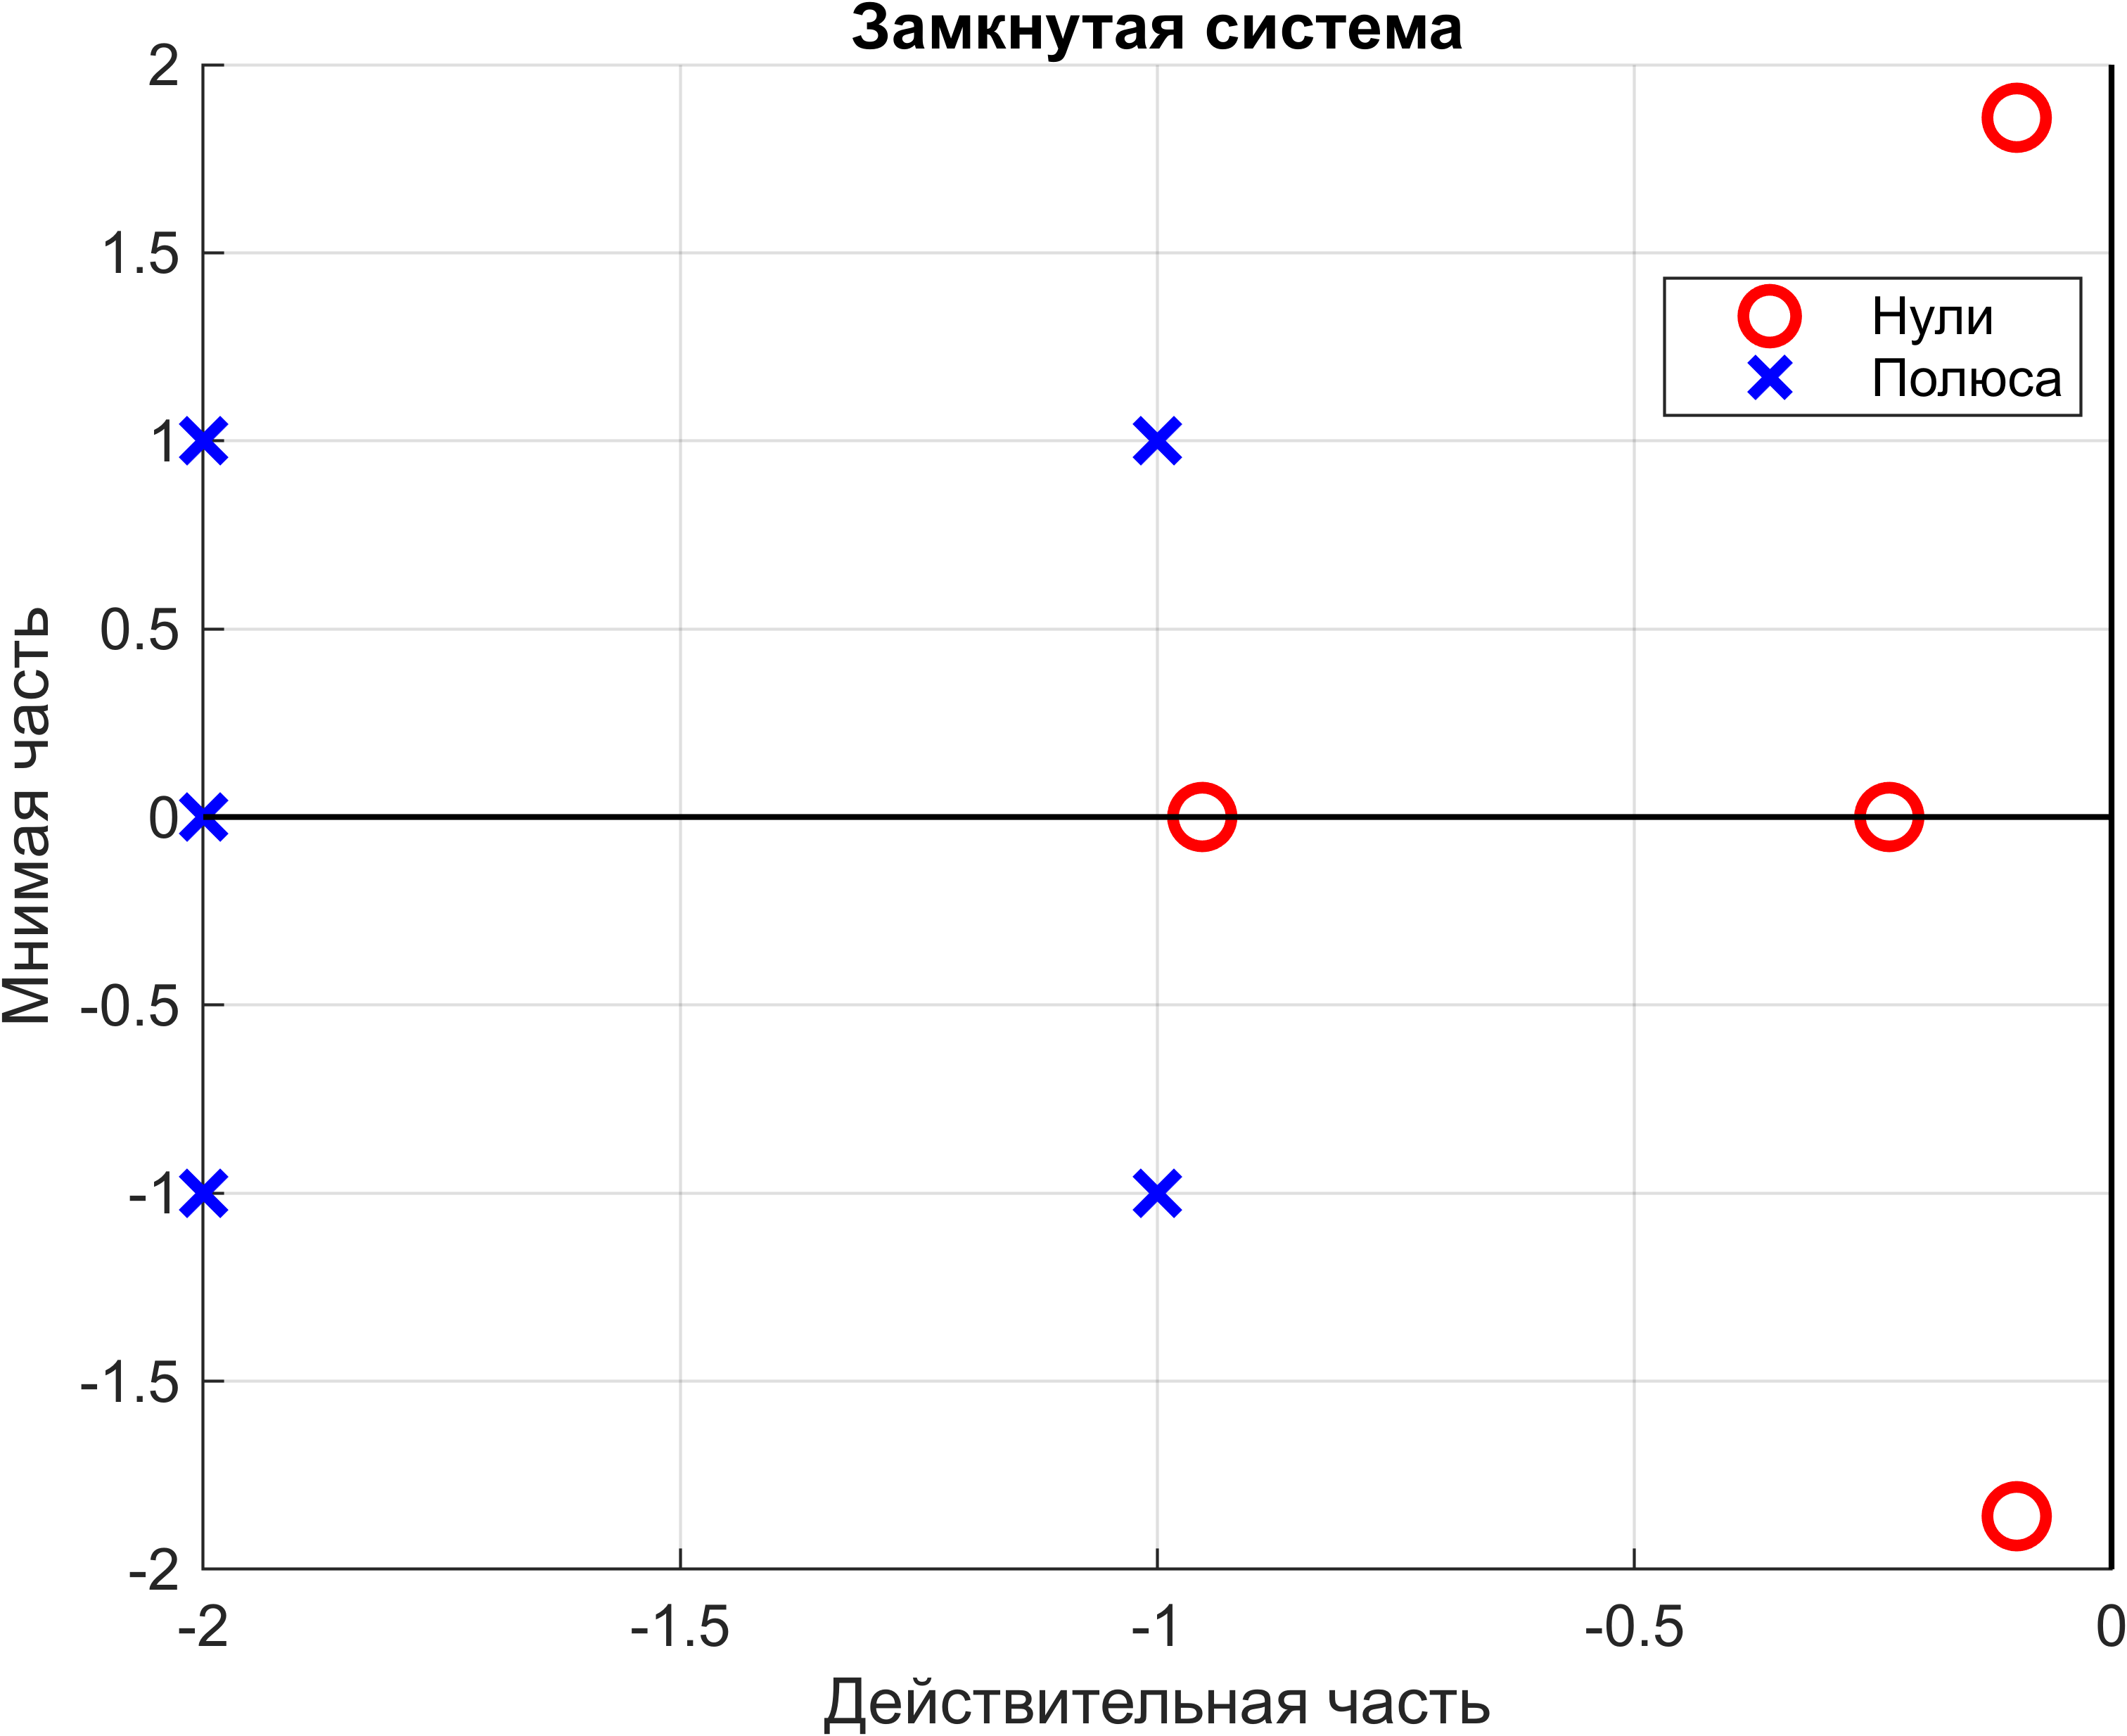
\includegraphics[width=1\textwidth, trim={0cm 0cm 0cm 0cm}]{../images/1_3_map_cl.png}
    \end{minipage}
    \caption{Карта полюсов и нулей разомкнутой и замкнутой системы}
\end{figure}

Построим переходные характеристики разомкнутой и замкнутой системы:
\begin{figure}[H]
    \centering
    \begin{minipage}{0.45\textwidth}
        \centering
        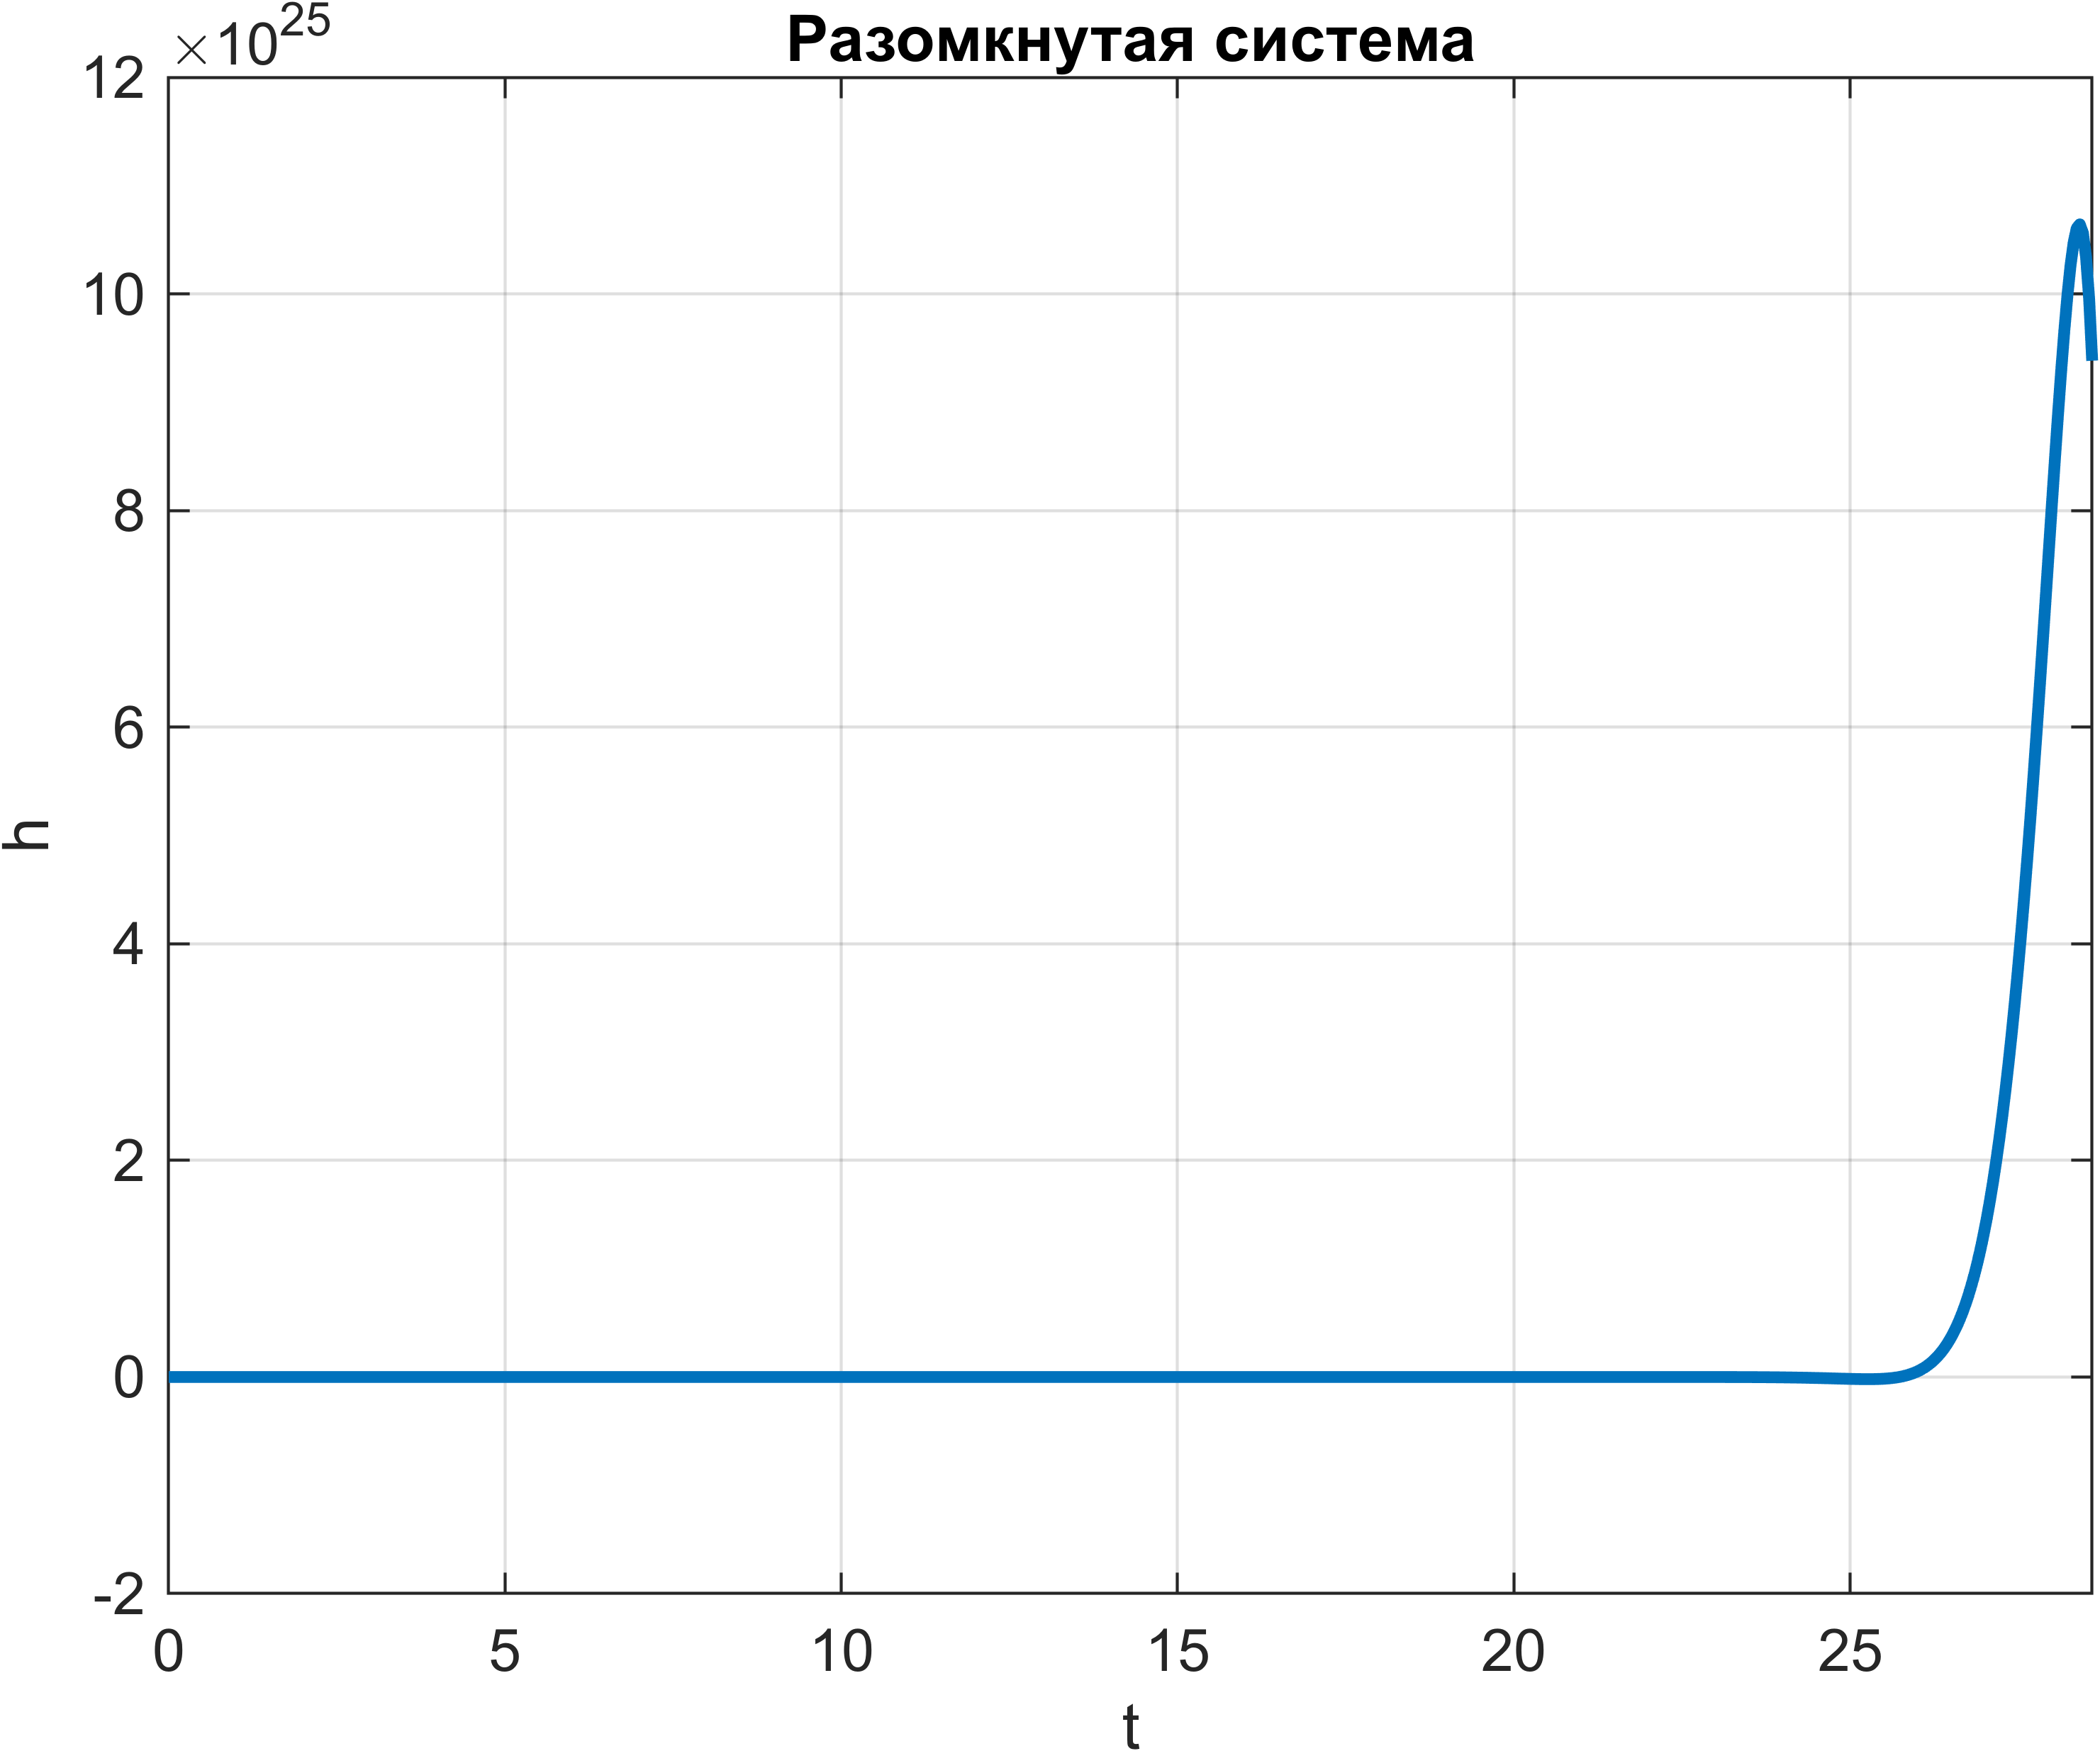
\includegraphics[width=1\textwidth, trim={0cm 0cm 0cm 0cm}]{../images/1_3_h_ol.png}
    \end{minipage}
    \hfill
    \begin{minipage}{0.45\textwidth}
        \centering
        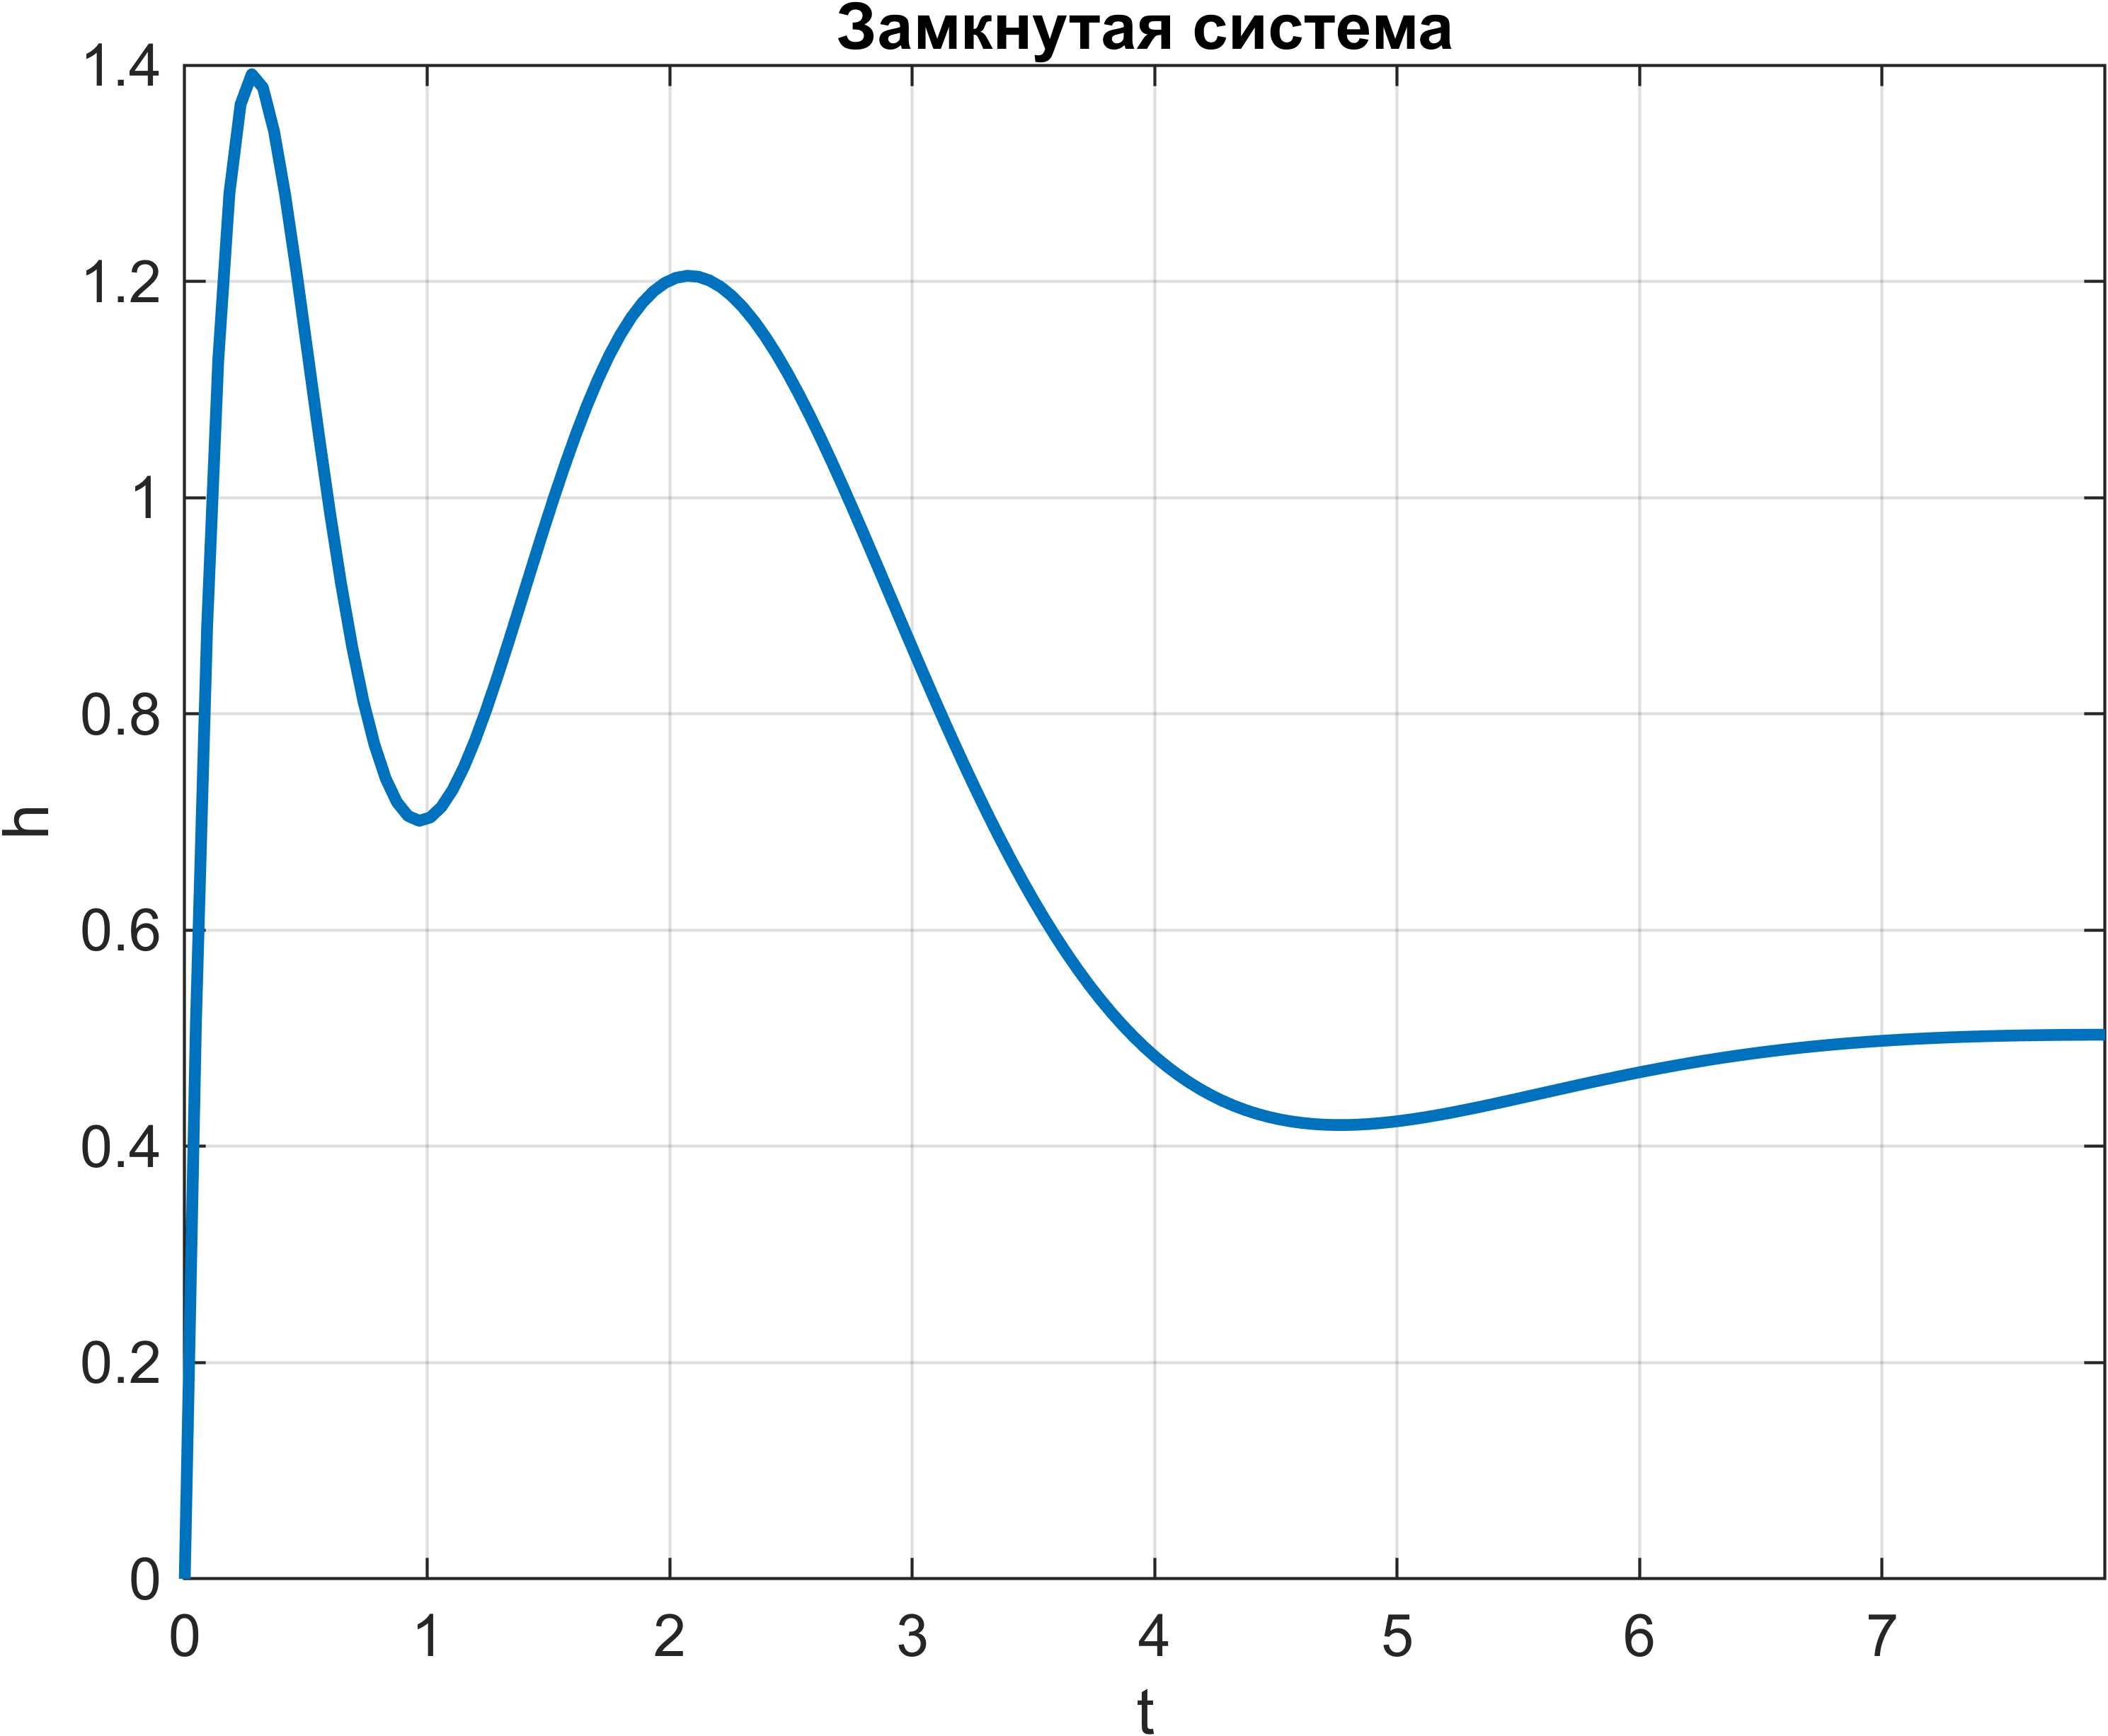
\includegraphics[width=1\textwidth, trim={0cm 0cm 0cm 0cm}]{../images/1_3_h_cl.png}
    \end{minipage}
    \caption{Переходные характеристики разомкнутой и замкнутой системы}
\end{figure}

Годограф Найквиста для данной передаточной функции:
\begin{figure}[H]
    \centering
    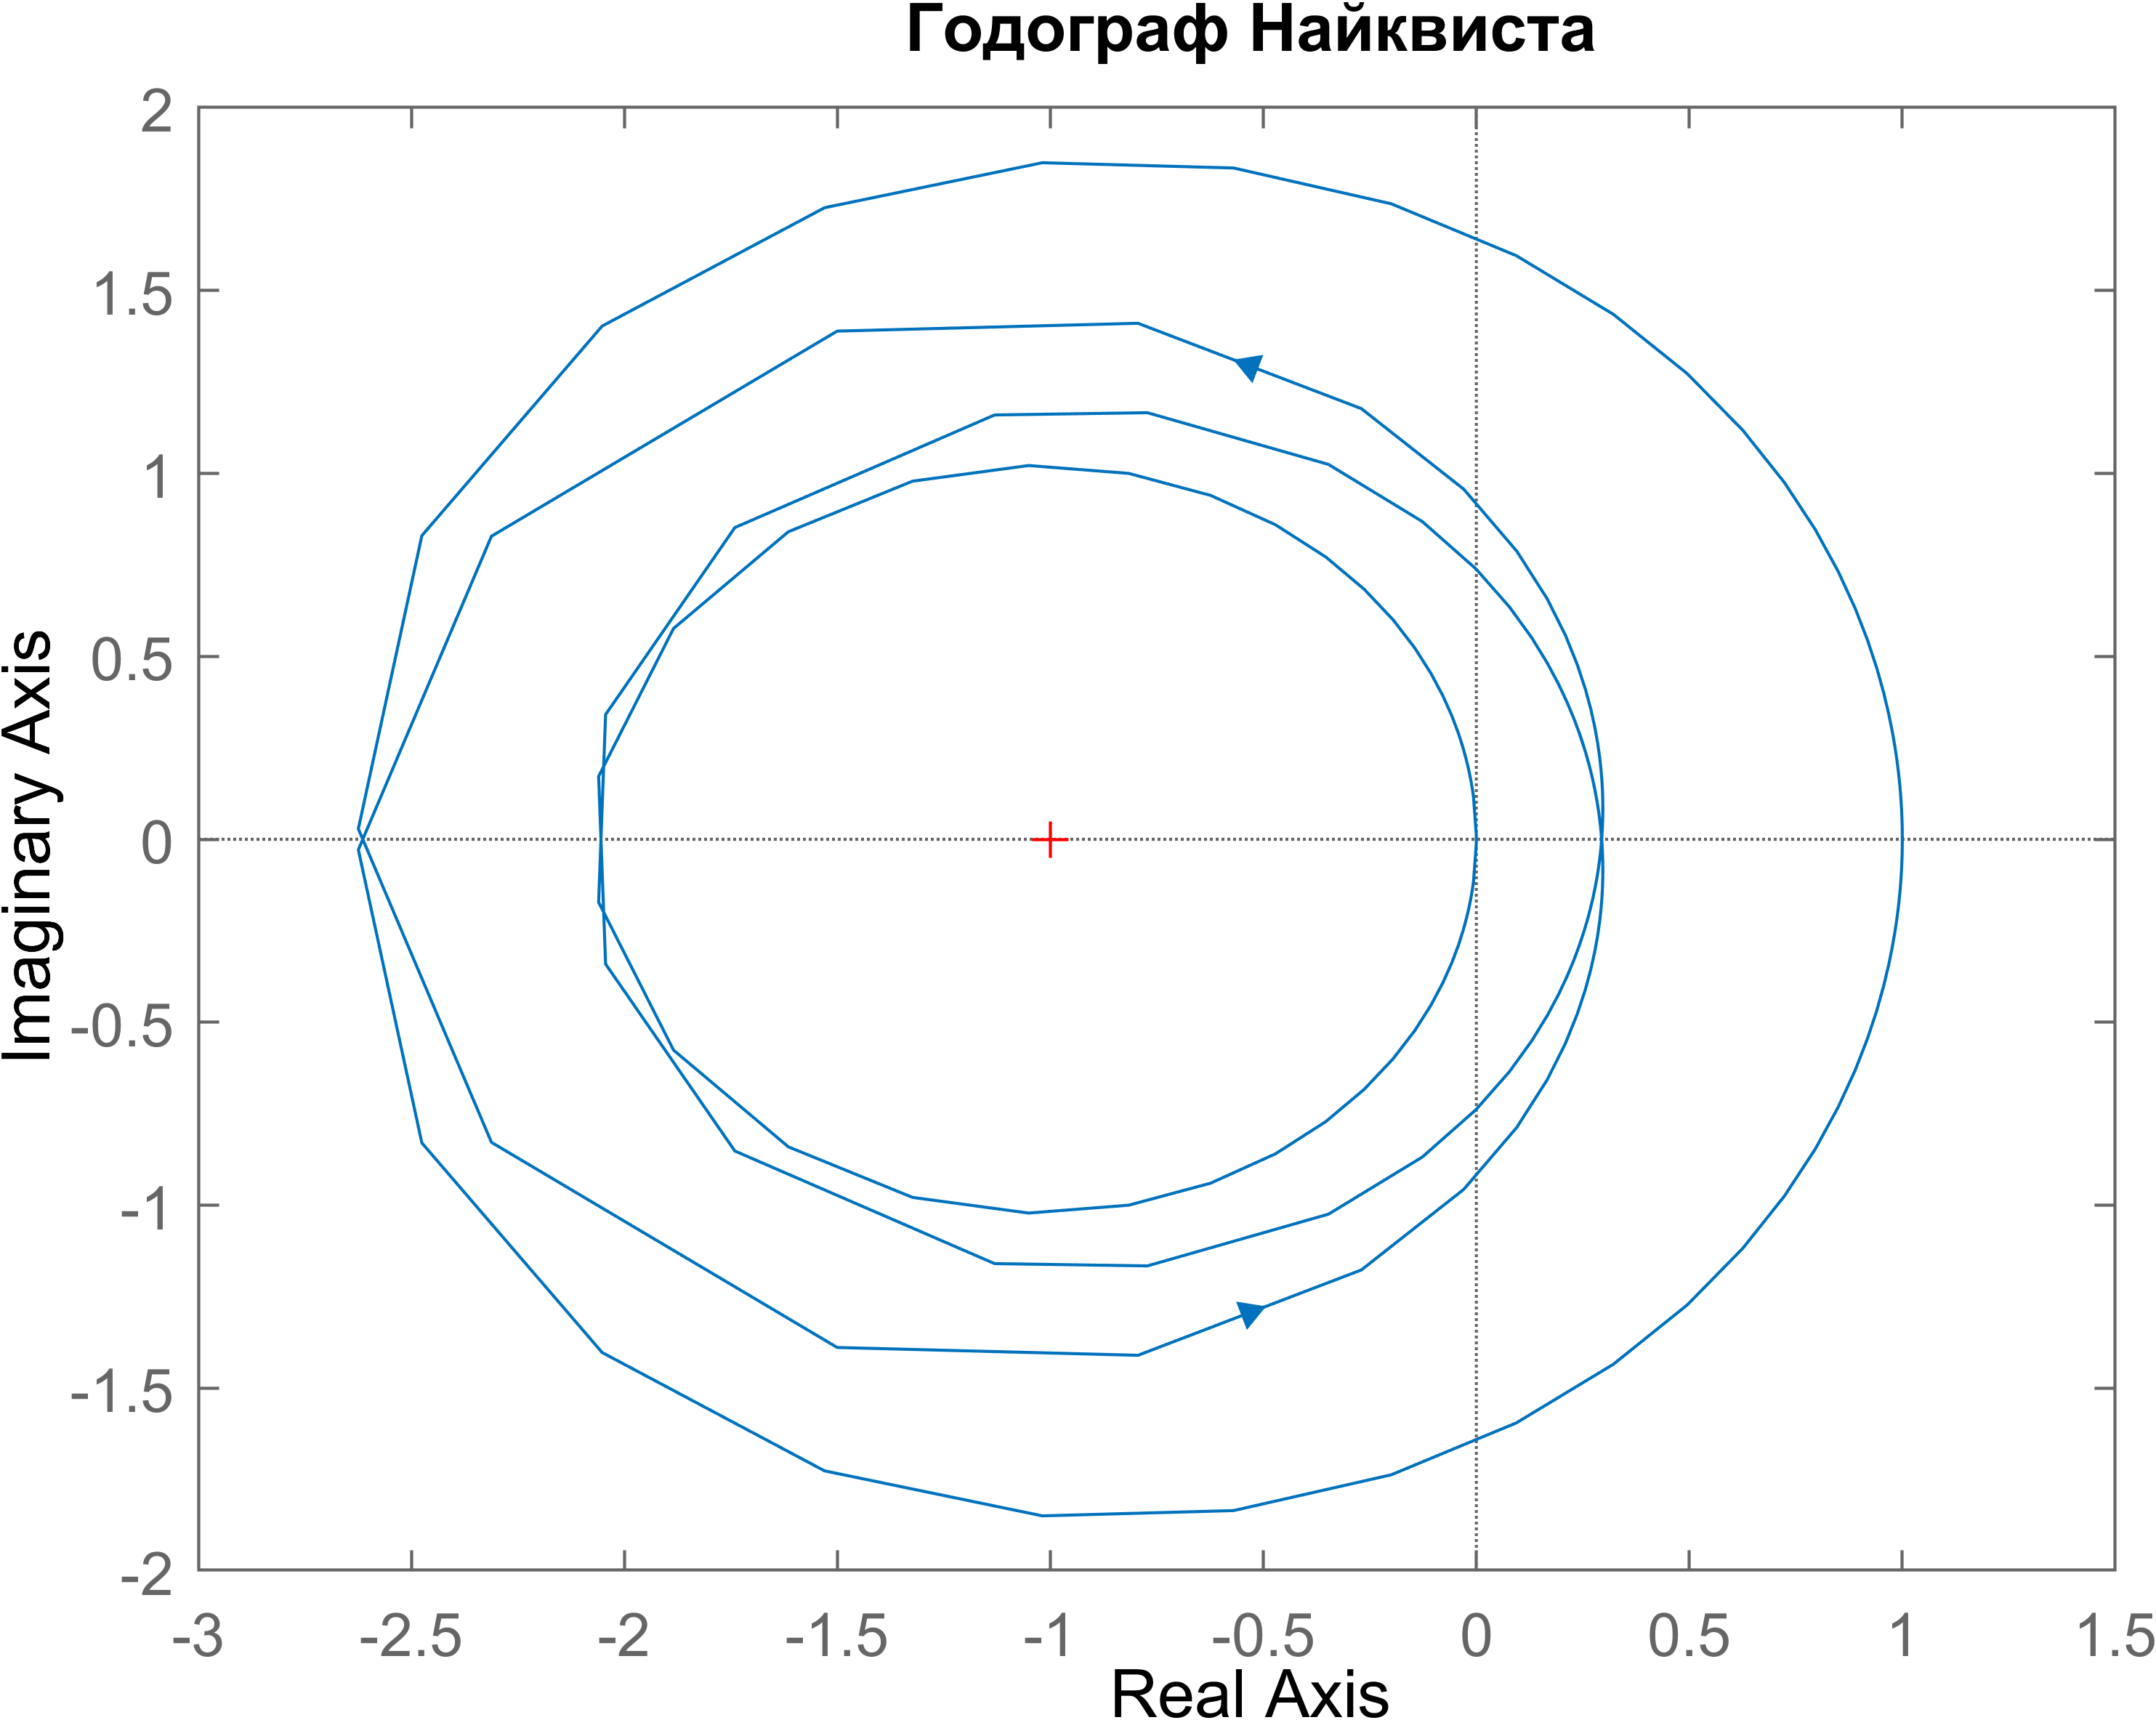
\includegraphics[width=0.7\textwidth, trim={0cm 0cm 0cm 0cm}]{../images/1_3_hod.png}
    \caption{Годограф Найквиста}
\end{figure}

Как видим, годограф совершил 4 оборота против часовой стрелки вокруг точки (-1, 0). Это соотносится с критерием Найквиста, так как
количество устойчивых полюсов уменьшилось на количество оборотов годографа при замыкании системы.

Рассмотрим ЛАФЧХ для данной передаточной функции:
\begin{figure}[H]
    \centering
    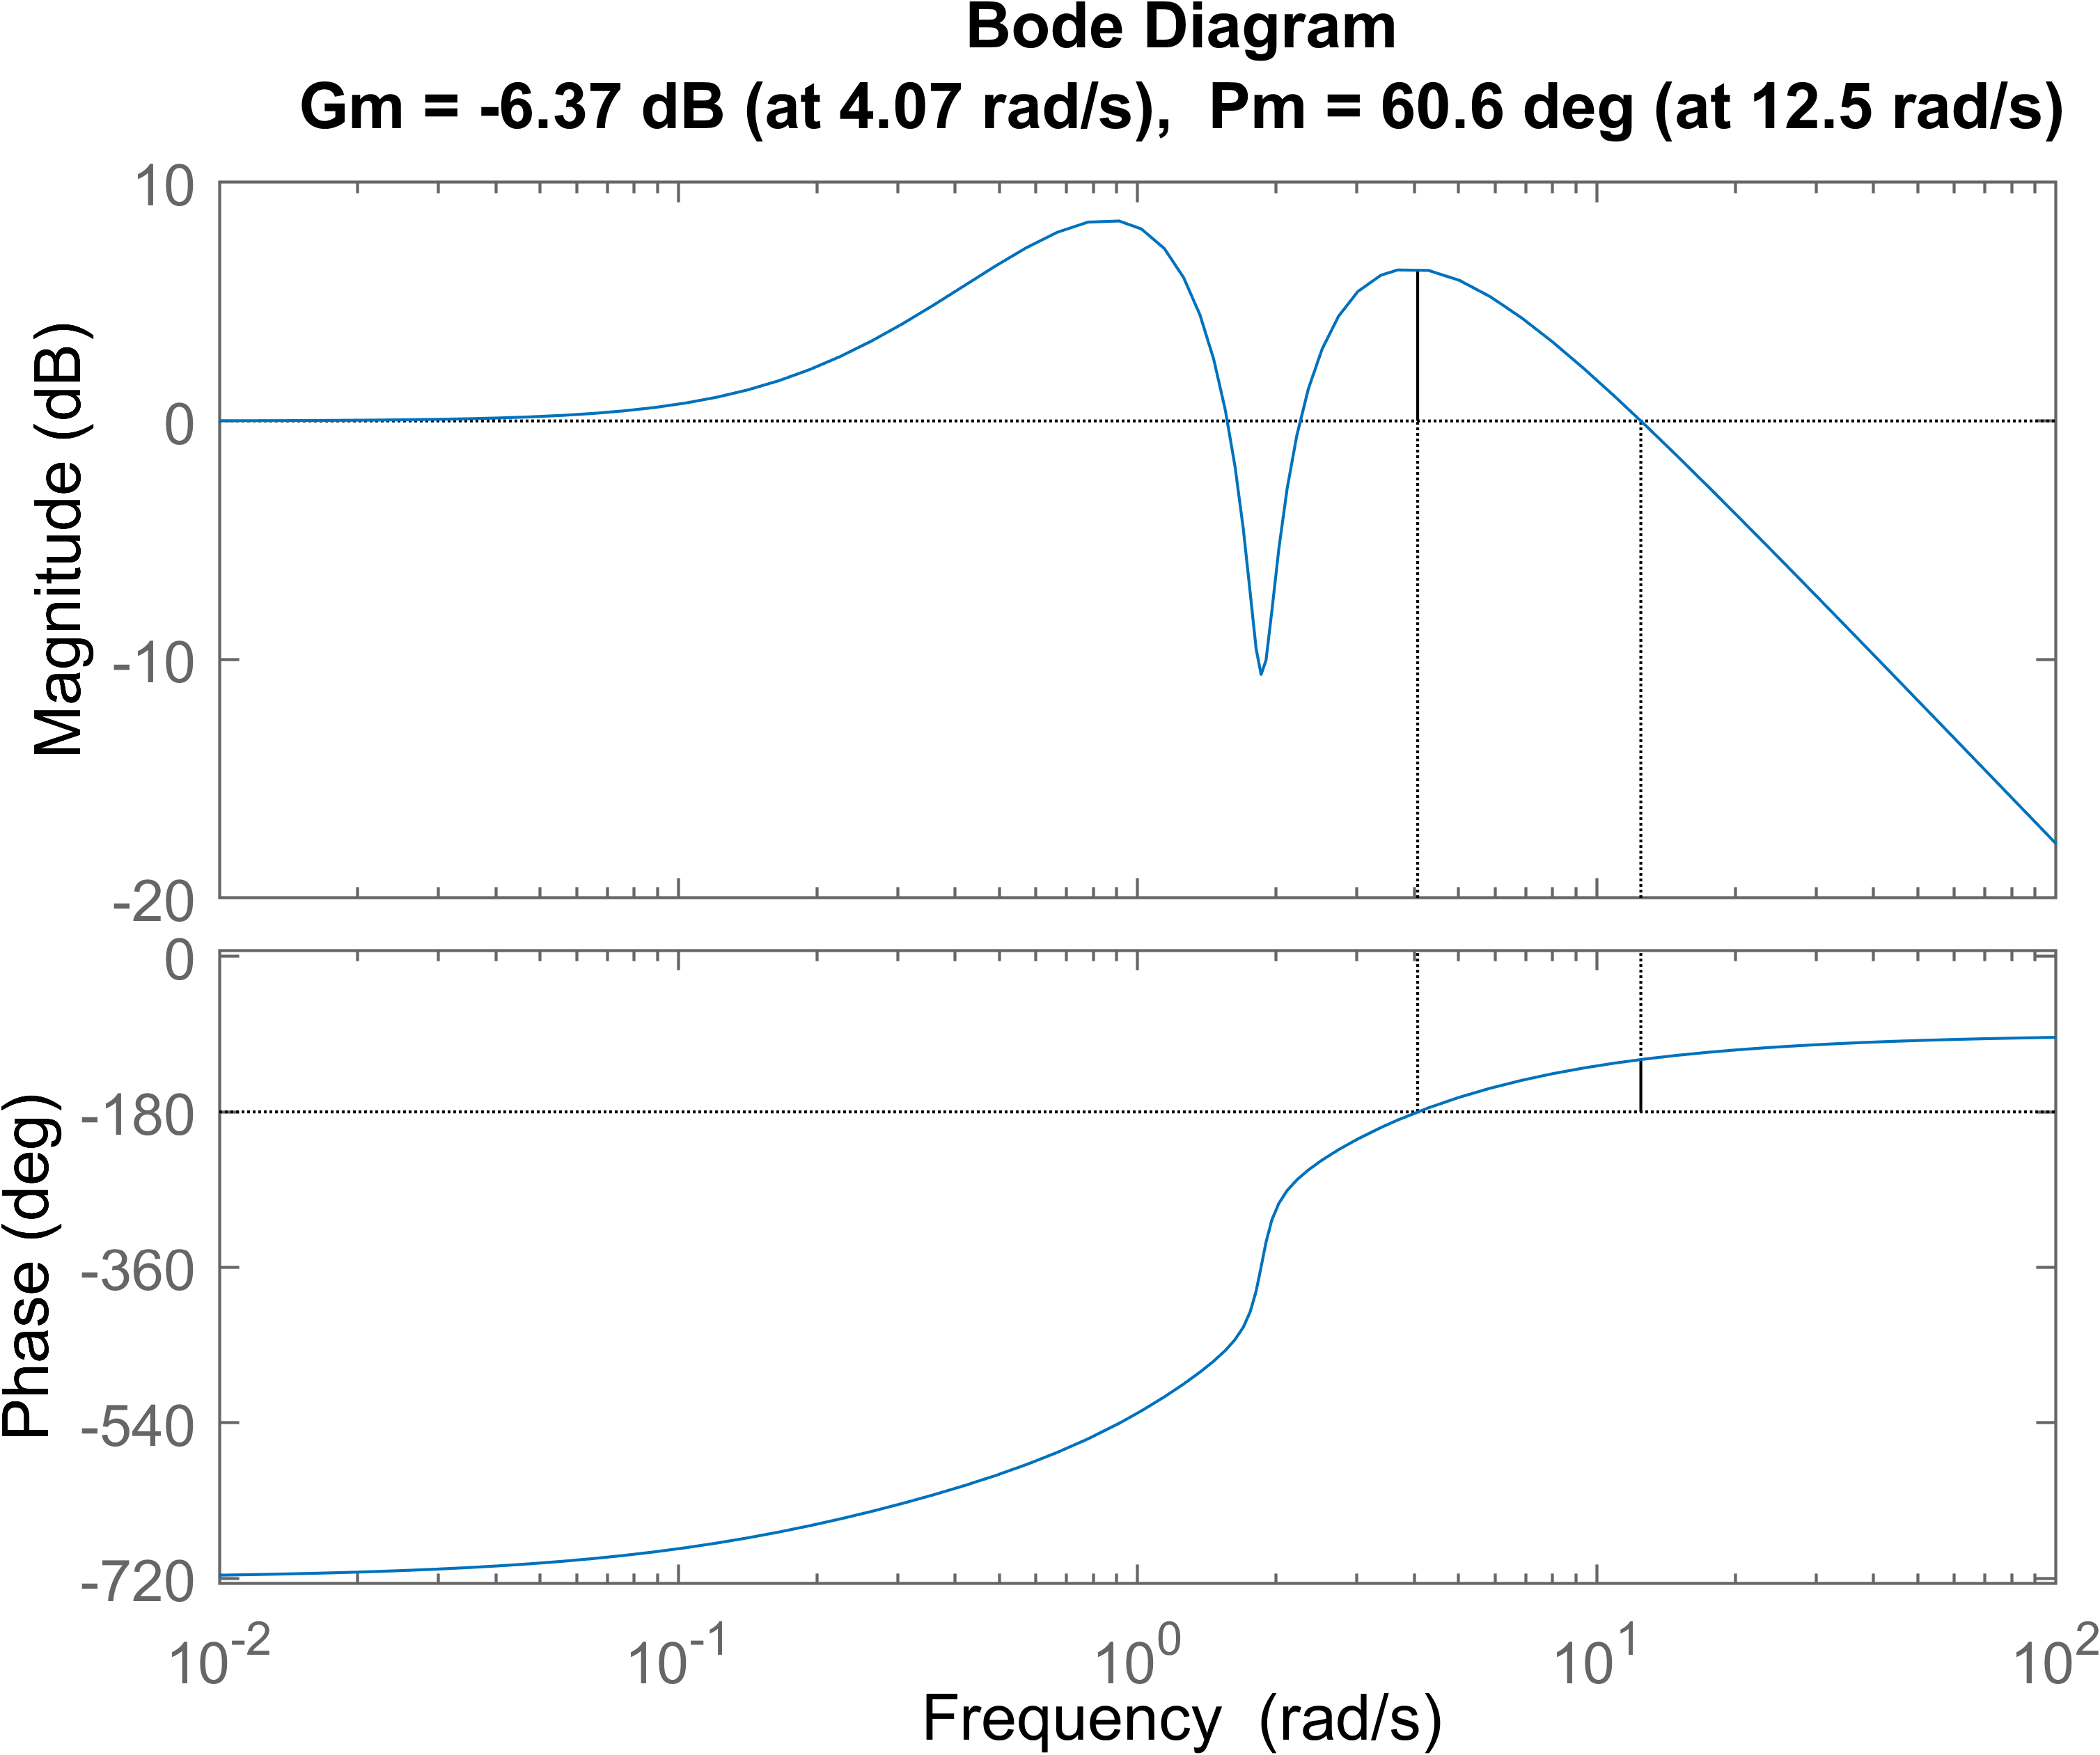
\includegraphics[width=0.7\textwidth, trim={0cm 0cm 0cm 0cm}]{../images/1_3_lapfs.png}
    \caption{ЛАФЧХ системы}
\end{figure}

ЛФЧХ имеет два положительных перехода (540 и 180 градусов), что соответствует устойчивости системы
, для которой нужна разность \(\frac{r}{2} = 2\).


\endinput